%%%%%%%%%%%%%%%%%%%%%%%%%%%%%%%%%%%%%%%%%
% Masters/Doctoral Thesis 
% LaTeX Template
% Version 2.3 (25/3/16)
%
% This template has been downloaded from:
% http://www.LaTeXTemplates.com
%
% Version 2.x major modifications by:
% Vel (vel@latextemplates.com)
%
% This template is based on a template by:
% Steve Gunn (http://users.ecs.soton.ac.uk/srg/softwaretools/document/templates/)
% Sunil Patel (http://www.sunilpatel.co.uk/thesis-template/)
%
% Template license:
% CC BY-NC-SA 3.0 (http://creativecommons.org/licenses/by-nc-sa/3.0/)
%
%%%%%%%%%%%%%%%%%%%%%%%%%%%%%%%%%%%%%%%%%

%----------------------------------------------------------------------------------------
%	PACKAGES AND OTHER DOCUMENT CONFIGURATIONS
%----------------------------------------------------------------------------------------

\documentclass[
11pt, % The default document font size, options: 10pt, 11pt, 12pt
%oneside, % Two side (alternating margins) for binding by default, uncomment to switch to one side
%chapterinoneline,% Have the chapter title next to the number in one single line
english, % ngerman for German
singlespacing, % Single line spacing, alternatives: onehalfspacing or doublespacing
%draft, % Uncomment to enable draft mode (no pictures, no links, overfull hboxes indicated)
%nolistspacing, % If the document is onehalfspacing or doublespacing, uncomment this to set spacing in lists to single
%liststotoc, % Uncomment to add the list of figures/tables/etc to the table of contents
%toctotoc, % Uncomment to add the main table of contents to the table of contents
%parskip, % Uncomment to add space between paragraphs
%nohyperref, % Uncomment to not load the hyperref package
headsepline, % Uncomment to get a line under the header
]{MastersDoctoralThesis} % The class file specifying the document structure

\usepackage[utf8]{inputenc} % Required for inputting international characters
\usepackage[T1]{fontenc} % Output font encoding for international characters

\usepackage{palatino} % Use the Palatino font by default

\usepackage[backend=biber,style=numeric,sorting=none]{biblatex} 
\addbibresource{example.bib} % The filename of the bibliography

\usepackage{listings} % For code listings
\usepackage{color}

\usepackage{enumitem}
\usepackage{tabularx}

\usepackage[autostyle=true]{csquotes} % Required to generate language-dependent quotes in the bibliography

%----------------------------------------------------------------------------------------
%	CODE LISTING SETTINGS
%---------------------------------------------------------------------------------------- 
\definecolor{codegreen}{rgb}{0,0.6,0}
\definecolor{codegray}{rgb}{0.5,0.5,0.5}
\definecolor{codepurple}{rgb}{0.58,0,0.82}
\definecolor{backcolour}{rgb}{0.95,0.95,0.92}
 
\lstdefinestyle{solidity}{
    backgroundcolor=\color{backcolour},   
    commentstyle=\color{codegreen},
    keywordstyle=\color{magenta},
    numberstyle=\tiny\color{codegray},
    %stringstyle=\color{codepurple},
    basicstyle=\footnotesize,
    breakatwhitespace=false,         
    breaklines=true,                 
    captionpos=b,                    
    keepspaces=true,                 
    %numbers=left,                    
    %numbersep=5pt,                  
    showspaces=false,                
    showstringspaces=false,
    showtabs=false,                  
    tabsize=2
}
 
\lstset{style=solidity}
%----------------------------------------------------------------------------------------
%	MARGIN SETTINGS
%----------------------------------------------------------------------------------------

\geometry{
	paper=a4paper, % Change to letterpaper for US letter
	inner=2.5cm, % Inner margin
	outer=3.8cm, % Outer margin
	bindingoffset=2cm, % Binding offset
	top=1.5cm, % Top margin`
	bottom=1.5cm, % Bottom margin
	%showframe,% show how the type block is set on the page
}

%----------------------------------------------------------------------------------------
%	HELPERS
%----------------------------------------------------------------------------------------

% Define some commands to keep the formatting separated from the content 
\newcommand{\keyword}[1]{\textbf{#1}}
\newcommand{\tabhead}[1]{\textbf{#1}}
\newcommand{\code}[1]{\texttt{#1}}
\newcommand{\file}[1]{\texttt{\bfseries#1}}
\newcommand{\option}[1]{\texttt{\itshape#1}}
\newcommand{\myworries}[1]{\textcolor{red}{#1}}

%----------------------------------------------------------------------------------------
%	THESIS INFORMATION
%----------------------------------------------------------------------------------------

\thesistitle{An Investigation of Re-decentralised Web Technology and its Possible Application for Cooperative governance} % Your thesis title, this is used in the title and abstract, print it elsewhere with \ttitle
\supervisor{Dr. Anandha \textsc{Gopalan}} % Your supervisor's name, this is used in the title page, print it elsewhere with \supname
\examiner{} % Your examiner's name, this is not currently used anywhere in the template, print it elsewhere with \examname
\degree{Master of Engineering} % Your degree name, this is used in the title page and abstract, print it elsewhere with \degreename
\author{Jack \textsc{Thorp}} % Your name, this is used in the title page and abstract, print it elsewhere with \authorname
\addresses{} % Your address, this is not currently used anywhere in the template, print it elsewhere with \addressname

\subject{Computing} % Your subject area, this is not currently used anywhere in the template, print it elsewhere with \subjectname
\keywords{} % Keywords for your thesis, this is not currently used anywhere in the template, print it elsewhere with \keywordnames
\university{\href{http://www.http://www.imperial.ac.uk/}{Imperial College London}} % Your university's name and URL, this is used in the title page and abstract, print it elsewhere with \univname
\department{\href{http://www.imperial.ac.uk/computing}{Department of Computing}} % Your department's name and URL, this is used in the title page and abstract, print it elsewhere with \deptname
%\group{\href{http://researchgroup.university.com}{Research Group Name}} % Your research group's name and URL, this is used in the title page, print it elsewhere with \groupname
\faculty{\href{http://faculty.university.com}{Faculty Name}} % Your faculty's name and URL, this is used in the title page and abstract, print it elsewhere with \facname

\hypersetup{pdftitle=\ttitle} % Set the PDF's title to your title
\hypersetup{pdfauthor=\authorname} % Set the PDF's author to your name
\hypersetup{pdfkeywords=\keywordnames} % Set the PDF's keywords to your keywords

\begin{document}

\frontmatter % Use roman page numbering style (i, ii, iii, iv...) for the pre-content pages

\pagestyle{plain} % Default to the plain heading style until the thesis style is called for the body content

%----------------------------------------------------------------------------------------
%	TITLE PAGE
%----------------------------------------------------------------------------------------

\begin{titlepage}
\begin{center}

{\scshape\LARGE \univname\par}\vspace{1.5cm} % University name
\textsc{\Large Project Report}\\[0.5cm] % Thesis type

\HRule \\[0.4cm] % Horizontal line
{\huge \bfseries \ttitle\par}\vspace{0.4cm} % Thesis title
\HRule \\[1.5cm] % Horizontal line
 
\begin{minipage}[t]{0.4\textwidth}
\begin{flushleft} \large
\emph{Author:}\\
\authorname % Author name - remove the \href bracket to remove the link
\end{flushleft}
\end{minipage}
\begin{minipage}[t]{0.4\textwidth}
\begin{flushright} \large
\emph{Supervisor:} \\
\href{https://www.doc.ic.ac.uk/~axgopala/}{\supname} % Supervisor name - remove the \href bracket to remove the link  
\end{flushright}
\end{minipage}\\[3cm]
 
\large \textit{A thesis submitted in fulfillment of the requirements\\ for the degree of \degreename}\\[0.3cm] % University requirement text
\textit{in the}\\[0.4cm]
\deptname\\[2cm] % Research group name and department name
 
{\large \today}\\[4cm] % Date
%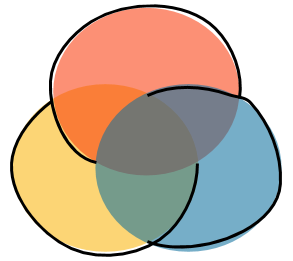
\includegraphics{Logo} % University/department logo - uncomment to place it
 
\vfill
\end{center}
\end{titlepage}
%----------------------------------------------------------------------------------------
%	ABSTRACT PAGE
%----------------------------------------------------------------------------------------

\begin{abstract}
\addchaptertocentry{\abstractname} % Add the abstract to the table of contents

This report is an exploration of the intersection of re-decentralised web technology and cooperative forms of organisation. We focus firstly on investigating the development of distributed web applications or 'dapps' using the Ethereum and IPFS platforms which includes a study of the practical technical  challenges to development and concerns around privacy and security. Then we investigate the governance processes of co-operative enterprises and discuss the specific challenge of maintaining member participation and representation at scale. Finally we present and evaluate Go-op a proof of concept application dapp for cooperative governance.

\end{abstract}

%----------------------------------------------------------------------------------------
%	ACKNOWLEDGEMENTS
%----------------------------------------------------------------------------------------

\begin{acknowledgements}
\addchaptertocentry{\acknowledgementname} % Add the acknowledgements to the table of contents

Special thanks go to my supervisor, Anandha Gopalan, for all his encouragement, understanding and enthusiasm, to my Dad, Robert, for his ongoing support and guidance and to my Family, for all their love.

\end{acknowledgements}

%----------------------------------------------------------------------------------------
%	LIST OF CONTENTS/FIGURES/TABLES PAGES
%----------------------------------------------------------------------------------------

\tableofcontents % Prints the main table of contents

\listoffigures % Prints the list of figures

\listoftables % Prints the list of tables

%----------------------------------------------------------------------------------------
%	THESIS CONTENT - CHAPTERS
%----------------------------------------------------------------------------------------

\mainmatter % Begin numeric (1,2,3...) page numbering

\pagestyle{thesis} % Return the page headers back to the "thesis" style

% Include the chapters of the thesis as separate files from the Chapters folder
% Uncomment the lines as you write the chapters

% Chapter 1

\chapter{Introduction} % Main chapter title

\label{Introduction} % For referencing the chapter elsewhere, use \ref{Chapter1} 


%----------------------------------------------------------------------------------------

\section{Motivation}
This report is an exploration of the intersection of two broad movements and the possibilities of social and technology system \cite{Sociotechnology} convergence through the specific application of blockchain technology to facilitate governance in cooperative organisations. The first "movement", comprises technical developers offering possible technical solutions to a range of social, economic, political and environmental challenges. These tech solutions currently fall within the emergent notion of Web 3.0. The second "movement", is a diverse socio-economic and political one concerned with shaping the emergent relationships between individuals and authorities, in a world recently interconnected by the internet. Both the technological and social developers in these areas are essentially focused on the rights of the individual, the terms on which they participate in social, economic, political and environmental domains.\\

\begin{figure}
\centering
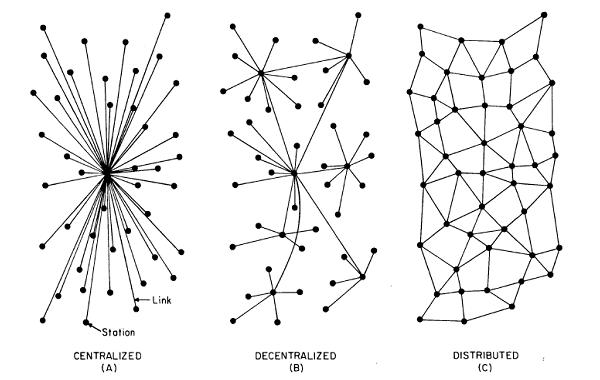
\includegraphics[width=\textwidth]{Figures/baran_net}
\decoRule
\caption[networks]{Centralized, Decentralized and Distributed Systems (Paul Baran, 1964)}
\label{fig:Electron}
\end{figure}

In 2014, on the 25th birthday of the World Wide Web, Tim Berners Lee listed his six goals for the future of the web:  re-decentralisation, openness, inclusion, privacy, free expression and security \cite{berners_lee}.  Despite enabling the hyper acceleration of that most fundamental of human activities: communication and, therefore, the speed at which we are now able to exchange not only information, but also values, the web has yet to fulfil the potential envisaged by it's creator.  The desire for openness, privacy, inclusion and free expression are typical concerns for the 'netizens' of today. \\

Over the past fifteen years, we have witnessed the explosion and monopolisation of web services and digital technology. The critical role of the web in modern society means that a handful of corporations now have alarming levels of political and economic power. \\

Netizens have sacrificed privacy for convenience and quality for control.\\

In this context, Snowden's revelations \cite{Snowden}, which implicate most of the 'internet giants' \cite{nsa_giants} (NSA's PRISM \cite{Prism} program and work with GCHQ to undermine encryption systems\cite{nsa_undermine}), has magnified growing tensions between the rights of citizens on the one hand and the "needs" of governments and corporations to control on the other. Distrust and dissatisfaction has pushed many developers and critics to propose alternative ways of constructing and organising the web, ways that are promoted as being truer to the dream of Tim Berners Lee. 

\subsection{Technical Solutions}
The trend for decentralised solutions, popularly referred to as Web 3.0, within the tech community can be observed from the emergence of new organisations (for example, redecentralize.org\cite{Redecentralise}, webwewant.org\cite{Webwewant}), new applications and services (for example, Firechat\cite{Firechat}, arkOS\cite{Arkos}, Solid\cite{Solid}, Mailpile\cite{Mailpile}) and even new hardware (for example, OPI\cite{OPI}, FreedomBox\cite{Freedombox}).\\

The most notable indicator however, is the recent rejuvenation of peer to peer systems. In the pure sense of the term\cite{p2pdef}, peer to peer networks are distributed systems by definition. The arrival of Bitcoin\cite{nakamoto2008bitcoin} dramatically increased the potential of peer to peer systems by introducing blockchains or distributed ledger technology (DLT). Blockchain networks allow peers to maintain a consistent view of shared data without the requirement for centralised authority. They are secure, transparent and far more resilient to attack and corruption than centralised alternatives.\\ 

The term Bitcoin 2.0 is now being used to describe a proliferation of new blockchain projects. One of the more established of these is Ethereum\cite{Ethereum}, a platform for building arbitrary applications on a blockchain.\\ 

In addition to blockchain networks, there are now also a number of peer to peer distributed file systems including IPFS (Inter Planetary File system \cite{Ipfs}), Maidsafe\cite{Maidsafe} and Storj\cite{Storj}. \\

The combination of blockchain platforms, distributed filesystems and other decentralised technologies is providing a framework for new forms of distributed web applications with significantly improved levels of availability, user control, security and privacy. \\

Designed in this way, services are also much more resilient to accidental, purposeful or environmental damage to the network (Consider the Google service dropout in 2013 resulting in 40\% drop of Internet traffic \cite{Google_outage}) and retrieving popular content, which is dynamically replicated across the network, is faster rather than slower. Efficient usage of bandwidth is particularly important given the increasing consumption of large data content (HD video etc), the networking of everything (Internet of Things, IoT) and the 4 billion users yet to come online\cite{Coming_online}.\\

Despite all the advantages a distributed web might bring, the tech community face a serious challenge of adoption. The 'internet giants' have established significant barriers to entry through the quality of their service offering. Providing a distributed alternatives it is understood will require a large amount of capital investment (ref Gupta?). \\

\subsection{Social Developments}
Characterising and describing current socio-economic "movements" attempting to imagine and build new social relationships in any detail is beyond the scope of this report. Broadly speaking, these movements (including, for example, P2P Foundation, opendemocracy, lasindias, community land trusts, "new economics") seem to be concerned with locating decision making close to those affected (distributed, decentralised), increasing participation and fairness (inclusivity), cooperation, transparency (openness) and sustainability. At the micro economic scale a number of business models have historically posed an alternative organisational alternative to the shareholder based private limited company, for example, worker and member cooperatives, Friendly or mutual benefit societies, trusts and more recently social enterprises and community interest companies. This report is focused on blockchain applications for cooperative enterprises. \\

Thus far the cooperative movement has failed to establish itself as a counterforce to narratives dominating the web and our new digital age that focus on brilliant ideas brought to market by Venture Capital. However, according to Michel Bauwens, of the P2P Foundation "cooperative enterprises are in the midst of a revival", that is "part of an ebb and flow of cooperativism, that is strongly linked to the ebb and flow of the mainstream capitalist economy."\cite{Open_cooperativism} \\

Included in this resurgence is the platform cooperativism initiative which promotes the restructuring of digital platforms as cooperative enterprises. In this spirit, issues of user control, privacy and security are tackled from a social perspective by reimagining the organisational forms of the 'centralised' service providers with a trusted, member controlled, inclusive alternative. \\

"The seeds are being planted for a new kind of online economy. For all the wonders the Internet brings us, it is dominated by an economics of monopoly, extraction, and surveillance. Ordinary users retain little control over their personal data, and the digital workplace is creeping into every corner of workers' lives." \cite{Platform_cooperativism}.\\


\subsection{Synthesis}
The founding proposition of cooperatives around the world is member participation in value creation and sharing. This applies equally at scale and whether the coop is "bricks and mortar" or an online platform.\\  

Fully engaging and mobilising members to participate has historically been problematic (see Myners\cite{Myners} for example) and raises serious questions about the best ways to create governance architecture that is fit for purpose. \\

One popular solution has been the creation of structures based around the election of "representatives" who mediate and aggregate individual member views to higher decision making levels. Historically, these governance architectures and their propensity to facilitate participation have been shaped by available information and communication technologies: the printed page and face to face social interactions. The resultant organisational structures have necessarily become hierarchical, not fully representative of the stakeholders, slow to execute decisions and open to the development of minority bias.\\

Digital information and communication technologies are changing the possibilities for social, economic and democratic participation and cooperation in all walks of life.\\

The first wave of Web 2.0 "social media" technologies have connected billions of people in new relationships. Facebook since 2003 has, for example, connected 1.5bn users. Many other applications (google drive, onedrive, icloud, yammer, slack, loomio etc) are built to enable "communities" to formally and informally cooperate and collaborate to create value and take decisions.\\

Web 3.0 or "re-distributed" web proposes concepts and tech that create new relationships between individuals, organisations and the data they create for mutual benefit. This is envisioned (see ref) as a shift from centralised to decentralised to distributed data.\\

The challenge for democratic member based economic or commercial enterprises is how to use these technologies and concepts to create competitive advantage using participative governance architectures that are trusted, secure, transparent, auditable, efficient and useable. \\

Conversely, the challenge for tech and digital communities is the harnessing of cooperative and solidarity organisational forms to develop quality web services that are able to compete with the incumbent offerings. \\

\section{Objectives}
Given the broad motivation, the objectives for this project have been threefold:
\begin{enumerate}
\item To investigate the Ethereum platform and surrounding technologies to develop insight into new forms of distributed web applications.
\item To develop an understanding of the state of the art and the practical and theoretical limitations of the technology.
\item To inform my investigation by developing a concrete application to address the governance challenges faced by new forms of global, distributed cooperative enterprises.
\end{enumerate}

\section{Contributions}
The contributions of the study are as follows:
\begin{itemize}
\item A first, proof of concept, Ethereum \& IPFS backed distributed application for co-operative governance called Go-op. Go-op allows co-operative members to establish and conduct governance on the Ethereum network. Co-operatives on Go-op can track membership, collect membership fees in Ether and table and vote on normal resolutions.
\item An in depth study into the emerging requirement for co-operative governance tools that can maintain member participation and representation at scale.
\item A detailed exploration and evaluation of the state of 'dapp' development using the Ethereum platform.
\end{itemize}



% Chapter 1

\chapter{Background} % Main chapter title

\label{Background} % For referencing the chapter elsewhere, use \ref{Background} 

\section{The Distributed Web}

\subsection{Blockchains}

\subsubsection{Introduction}
Since the 70's the modus operandi for data encapsulation and management has been SQL (Structured Query Languages) and RDBMS (Relational Database Management Systems). The 90's marked the arrival of the web, mass adoption of the Internet and networking of such database systems all over the world. However, because information is encapsulated in organisation centric forms, there are great inefficiencies communicating it over the network. Data sits in 'silos' and transferring it often requires an inevitable amount of bureaucracy and cost. In this context Blockchain technology offers an alternative approach to information storage. A global database that allows data to exists between organisations. So what are they? (see Vinay \cite{VinayOnBlockchains} for more on blockchains in context) \\

The concepts of a 'blockchain',  'blockchain technology' and 'distributed ledger technology' were first proposed and implemented by the Bitcoin electronic cash system, 2009\cite{nakamoto2008bitcoin}. The terms are used somewhat interchangeably to describe a peer to peer (and therefore decentralised) system that is capable of maintaining shared state in a way that is transparent, secure, permanent and resistant to corruption or attack. Within the Bitcoin cryptocurrency network, blockchains are used to maintain a globally consistent notion of account balances. There are now many more blockchain applications ranging from DNS registries (such as Namecoin\cite{Namecoin}) to alternative crypto currencies or ?altcoins? (such as LiteCoin\cite{Litecoin}, FairCoin\cite{Faircoin}, DogeCoin\cite{Dogecoin}) and even identity management systems (such as Onename\cite{Onename}). \\

The term blockchain is somewhat ambiguous in that it is often used interchangeably to describe both a data structure and a form of distributed database at the same time. A good description would perhaps make the distinction between a) a blockchain network - a peer to peer network that maintains distributed consensus on a blockchain data structure and b) a blockchain - the data structure that is stored by each peer (and therefore replicated across the entire network). Two things of important note are: Firstly the blockchain structure of the shared data is inextricable from the mechanisms used to maintain consensus of that data itself (this is a confusing statement that will be expanded upon shortly). Secondly, the comparison of blockchains to databases is conceptual. To be clear, a blockchain is not a relational database and there is no query language such as SQL. Further to this, sharding of blockchain data is uncommon in practise which is not generally the case in most other distributed database systems\cite{Shard}. \\

\begin{figure}
\centering
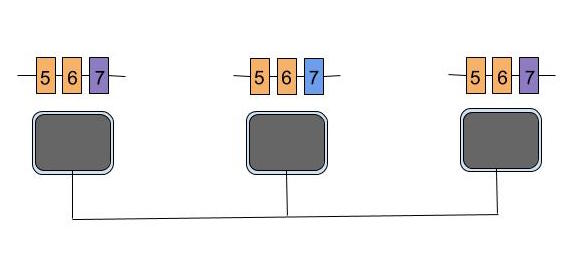
\includegraphics[width=\textwidth]{Figures/basic_chain}
\decoRule
\caption[Simplified Blockchain Network]{A simple illustration of a blockchain network with three peers.}
\label{fig:basic_chain}
\end{figure}

Figure \ref{fig:basic_chain} is an illustration of a simplified blockchain network. Each peer (grey box) has an almost identical full copy of the blockchain. Disagreement on final blocks is called 'forking'. Eventually all peers will agree on the same value for block 7. The type of consistency a blockchain network maintains is dependent on the number of blocks the observer chooses to discard from the end of the chain\cite{Bitcoin_consistency}. \\

\subsubsection{Transactions and Blocks}
Blockchain networks provide both read and write functionality. For the purposes of this discussion a transaction is a network input that results in a write to the blockchain. Whilst a read request may be fulfilled by any network peer, transactions must be processed by the entire network. For example, a payment in Bitcoin is a transaction. It causes a write to the blockchain as a change in account balances. \\

A block is a collection of transactions. The first block in a blockchain is called the genesis block. Each block thereafter represents a discrete update to the shared state. \\

\subsubsection{Blockchains as State Transition Systems}
A good approach to explaining blockchains is as state transition systems. State transition functions and finite state machines are familiar concepts to computer scientists. In a blockchain we can say that the history of the chain (i.e all previously processed transactions) encapsulates the state of the system. The addition of a new block, updates that history and therefore transitions the blockchain to a new state. This idea is illustrated in Figure \ref{fig:blockchain_transition} \\

\begin{figure}
\centering
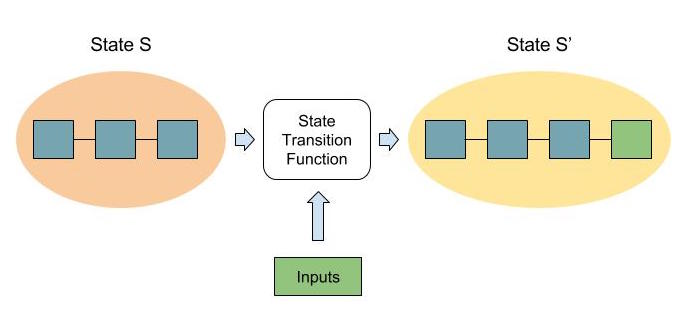
\includegraphics[width=1.4\textwidth]{Figures/blockchain_transition}
\decoRule
\caption[Blockchain As State Transition]{Conceptualisation of a blockchain as a state transition system.}
\label{fig:blockchain_transition}
\end{figure}

The state may be encapsulated by the history of the blockchain in many ways. For instance, in the Bitcoin network the state is the sum of each user's unspent bitcoins i.e all account balances. A user's balance is derived by scanning through every previous block to find all received Bitcoins that have not yet been spent (users spend specific coins through the concept of unspent transaction outputs). This is not the case in the Ethereum network (discussed later) in which a user's balance is explicitly stored in every block (i.e no scanning operation required). An example state transition for a Bitcoin network is given in Figure \ref{fig:bitcoin_transition}. There are five unspent transaction outputs in the initial state. The transaction uses two of these to make three payments. This results in a new state with six unspent transaction outputs. \\

\begin{figure}
\centering
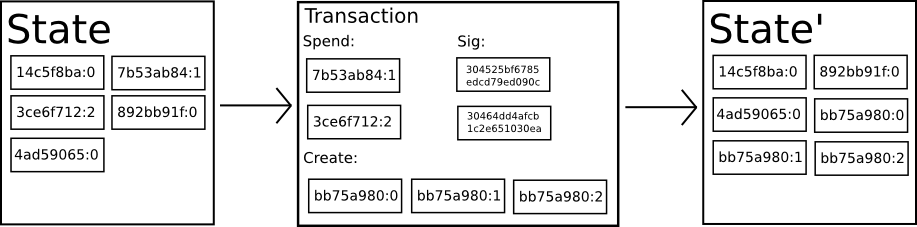
\includegraphics[width=1.4\textwidth]{Figures/state_transition}
\decoRule
\caption[Bitcoin State Transition]{Bitcoin state transition diagram (taken from the Ethereum Whitepaper\cite{Ethereum})}
\label{fig:bitcoin_transition}
\end{figure}

The state transition function for a cryptocurrency like bitcoin might go something like:
\begin{enumerate}
\item Check each referenced or spent bitcoins (unspent transaction outputs) are available in the start state.
\item Check transaction signature is same as the bitcoin owner
\item Check sum of input bitcoins is at least equal to sum of output bitcoins.
\item Return new state 
\end{enumerate}

\subsubsection{Blockchain mining}
Mining is the process through which new blocks are created and distributed across the network. The general process proceeds something like the following:
\begin{enumerate}

\item A network peer creates or collects transactions (i.e state changing inputs).


\item A block header is created containing a number of fields. This includes the hash of the previous block (which creates a link in the chain), the block difficulty, a timestamp and a compressed, unique identifier, for the transaction set e.g a merkle\cite{Merkle} tree root.


\item The peer generates a proof of work. A typical proof of work involves repeatedly hashing\cite{Hash} the block header, varying a small amount of data each time (called the nonce) until a hash is produced with some agreed characteristics. One example is X amount of leading zeros (X is then the block difficulty).


\item The inputs (from step 1) and the block header (from step 2) form a block which is broadcast to the rest of the network. 


\item Peers receiving the block 

\begin{enumerate}
\item Check the hash of the previous block is valid

\item Validate the new state. Apply the block transactions to their current state (using the particular state transition function of the system) to check they are correct.

\item Add the block to their chain.
\end{enumerate}
\end{enumerate}

\begin{figure}
\centering
\makebox[\textwidth][c]{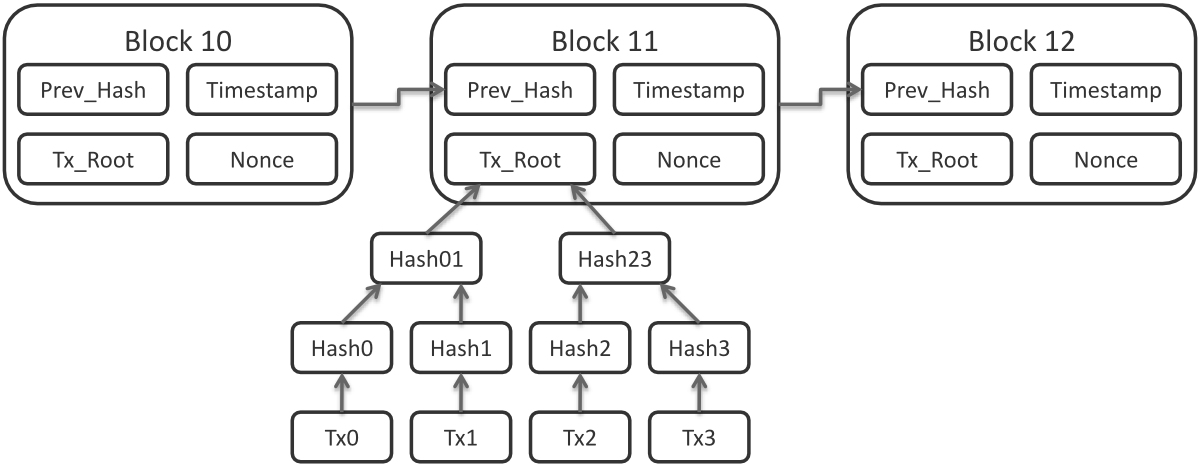
\includegraphics[width=1.4\textwidth]{Figures/blockchain}}
\decoRule
\caption[Sequence of Blockchain Headers]{A section of blockchain headers. Illustration by Matthaus Wander (Wikimedia) \cite{blockchainHeaders}}
\label{fig:bitcoin_transition}
\end{figure}

\subsubsection{Proof of work, hash functions and security}
The use of hash functions in both the compression of transactions in step 2 and the generation of a proof of work in step 3 are crucial to the security and consensus mechanisms of blockchain systems.\\

Any change to the input of a hash function results in a change in the output. Finding an input to a hash function that results in a given output is incredibly difficult and only achievable through a  brute force approach. This has two important implications.\\

Firstly, a proof of work (e.g generate hash with X leading zeros) can only be found through a trial and error approach. This establishes a formal economic barrier (electricity cost of CPU cycles) that limits the ability of any peer to add a new block to the chain. \\

Secondly, any change to a transaction in a previous block would result in a new transaction hash, which in turn would change the transaction root which in turn would change the block header. This would invalidate both the proof of work for that block and the previous hash link used in the next block. \\

This makes it impossible to change any transaction in the history of the chain without redoing the proof of work for every subsequent block. Such an undertaking is computationally infeasible for any group (colluding or otherwise) that cannot produce blocks faster than the rest of the network. In the case of most public blockchains this would require significant capital resource. \\

\subsubsection{Incentivisation} 
The maintenance of blockchain networks requires the incentivised participation of miners. Whilst this may not necessarily be economic, most public blockchain systems (including Bitcoin and Ethereum) have some form of mining reward and/or transaction fee to allow miners to collect a direct monetary reward for producing blocks.\\

\subsubsection{Forks and consensus}
When multiple blocks are produced in quick succession, network latency can cause the forking of blockchains. Figure \ref{fig:basic_chain} is a simple example of a fork. \\

At some point, one partition of the network will become aware of a longer chain being mined by another partition. Because this chain is longer, it contains a greater amount of work and is more likely to be accepted by the rest of the network. Miners are incentivised to work on the chain that is most likely to be adopted by the rest of the network because it increases the chance that their reward for creating blocks will be permanent.\\

\subsubsection{Proof of Stake}

\subsubsection{Sharding}

\subsubsection{Value Proposition}

\subsection{Ethereum}
\subsubsection{Introduction}
Ethereum is a public blockchain platform for running arbitrary applications with extremely low possibility of downtime, censorship, fraud or third party interference. It is a peer to peer network that stores turing complete programs within a blockchain. It has been described as a 'global computer' and a 'globally executed virtual machine'. The idea was first proposed by Vitalik Buterin who formally unveiled the project at the Miami Bitcoin Conference in early 2014. Later that year Ethereum is estimated to have raised over 20 million dollars in less than a month, making it one of the most successful crowdfunds ever\cite{Ethereum_crowdfund}. \\

The previous section of this report described how blockchains can be considered as state transition systems. The state transition function of Ethereum works by executing turing complete programs that are stored in the blockchain itself. In this sense it is perhaps the most general blockchain system conceivable. Bitcoin, Namecoin and Coloured Coins could all be implemented as contract code executing on the Ethereum blockchain. Buterin has described it as "The ultimate foundational layer"\cite{Ethereum}. \\

Although the state transition system may be very innovative, the fundamental consensus and proof of work mechanisms are very similar to other blockchain networks. The Ethereum platform still needs to incentivise miners and for this purpose has it's own internal cryptocurrency called Ether. \\

The rest of this subsection provides an introductory explanation to the Ethereum protocol. A more complete introduction has been written by Buterin\cite{Ethereum} and a comprehensive technical specification has been written by Wood\cite{wood2014ethereum}. Practical information and references for navigating the Ethereum ecosystem can be found in Appendix Y. \\

\subsubsection{Ethereum Accounts}
There are two types of accounts in Ethereum: \keyword{externally owned accounts} and \keyword{contract accounts}. \\

\begin{figure}
\centering

\includegraphics[width=\textwidth]{Figures/ethereum_accounts}
\decoRule
\caption[Ethereum Accounts]{Illustration of the two different types of Ethereum accounts}
\label{fig:ethereum_accounts}
\end{figure}

Externally owned accounts are effectively user accounts. They are controlled by private keys and have a balance in Ether. Contract accounts also have a balance but unlike externally owned accounts they also have code and storage. Contract accounts are controlled by their code. Both types of account are able to form transactions to both send Ether and call contract code.\\

\subsubsection{Ethereum as a state transition system}
Given this notion of accounts, the state of the Ethereum network is the aggregated state of each individual account. \\

Transactions are then either a) a direct transfer of ether between any pair of accounts, b) a contract creation request or c) a call to a contract method with a collection of argument parameters. Respectively, applying these transactions to the old state then either a) increases and decreases balances, b) adds a new account to the state or c) updates contract storage according to the execution of program code in the Ethereum virtual machine (EVM). \\

Unlike Bitcoin, where blocks simply contain a set of transactions, blocks in the Ethereum blockchain contain a copy of both the transaction list and the new state (balances, storage etc of all accounts). This account based approach, where the state is stored in every block, can seem more intuitive than that of unspent transaction outputs where state is derived through scanning the blockchain.\\

The consequence of storing the entire state in each block is that it is potentially inefficient in terms of storage. However, because most accounts do not change between blocks, a special type of merkle tree, called a patricia tree, is used so that data can be stored once and referenced multiple times ( a description of patricia trees is beyond the scope of this report but the interested reader should consult the Ethereum wiki \cite{Patricia}).\\

\begin{figure}
\centering
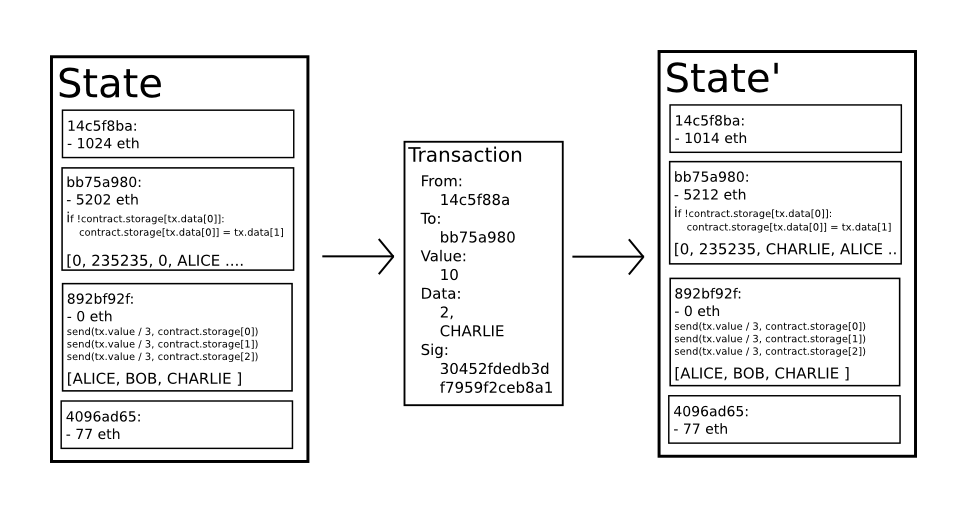
\includegraphics[width=\textwidth]{Figures/ethereum_transition}
\decoRule
\caption[Ethereum State Transition Diagram]{Ethereum State Transition Diagram}
\label{fig:ethereum_transition}
\end{figure}

Figure \ref{fig:ethereum_transition} shows an example state transition in the Ethereum blockchain. The initial state contains four accounts; two externally owned (user) accounts and two contract accounts. The transaction is a call from the first user account to execute code in the first contract account with the arguments 2 and CHARLIE and an ether value of 10. In the resultant state, the balance of the user account has decreased by 10, the balance of the contract account has increased by 10 and the storage of the contract account has changed according to the execution of its code with the given arguments.\\

\subsubsection{Gas}
Any Ethereum transaction contains a STARTGAS and GASPRICE parameter. Startgas specifies a limit to the number of computational steps the sender is willing to pay for during code execution. The gasprice specifies the amount, in wei (a sub denomination of ether), they are willing to pay for each unit of computation. Unlike some other blockchain networks, transactions in Ethereum consume different amounts of computational resources; consider a simple ether payment vs execution of a complex insurance contract. By making agents pays proportionally for the resources they consume it becomes impossible to form denial of service attacks via infinite looping (possible given turing completeness of contract code). \\

The miner of a block collects the gas funds, therefore the gasprice functions in a similar way to transaction fees. The greater the gasprice the more incentive there is for a miner to include that transaction within a block. Any gas remaining after the execution of a transaction is returned to the sender.\\ 

\subsubsection{Blockchain Mining}
\begin{figure}
\centering
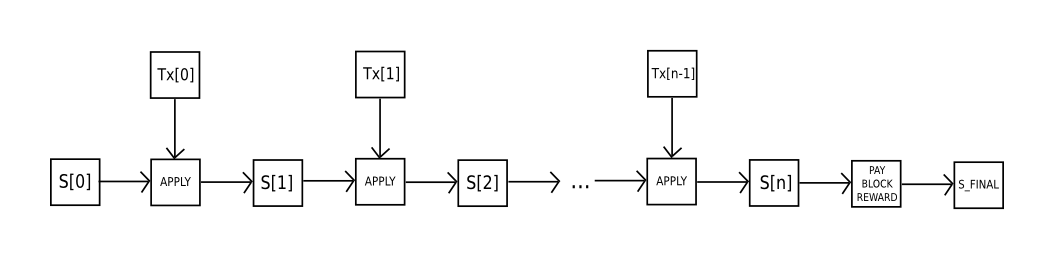
\includegraphics[width=\textwidth]{Figures/ethereum_state_transition}
\decoRule
\caption[Ethereum Block Validation Process]{Ethereum block validation process.}
\label{fig:ethereum_state_transition}
\end{figure}
The mining process of Ethereum is similar to the general blockchain process discussed in the previous section. The following steps describe the Ethereum block validation process as described in the Ethereum whitepaper (APPLY function executes transition function as above):

\begin{enumerate}
\item Check if the previous block referenced exists and is valid.


\item Check that the timestamp of the block is greater than that of the referenced previous block and less than 15 minutes into the future


\item Check that the block number, difficulty, transaction root, uncle root and gas limit (various low-level Ethereum-specific concepts) are valid.


\item Check that the proof of work on the block is valid.


\item Let S[0] be the state at the end of the previous block.


\item Let TX be the block's transaction list, with n transactions. For all i in 0...n-1, setS[i+1] = APPLY(S[i],TX[i]). If any application returns an error, or if the total gas consumed in the block up until this point exceeds the GAS LIMIT, return an error.


\item Let S\_FINAL be S[n], but adding the block reward paid to the miner.


\item Check if the Merkle tree root of the state S\_FINAL is equal to the final state root provided in the block header. If it is, the block is valid; otherwise, it is not valid.

\end{enumerate}

This process implies that every peer must eventually execute any contract code called by a transaction in order to check the validity of a new block. This is the reason Ethereum is often described as a 'globally executed virtual machine'.

\subsubsection{Smart Contracts}
In the context of Ethereum, programs stored in the blockchain are primarily referred to as smart contracts. Accounts that store code are called 'contract accounts'. The concept has a much broader definition outside of this context and was actually coined by Nick Szabo as early as 1993. According to Szabo "A smart contract is a computerized transaction protocol that executes the terms of a contract. The general objectives of smart contract design are to satisfy common contractual conditions (such as payment terms, liens, confidentiality, and even enforcement), minimize exceptions both malicious and accidental, and minimize the need for trusted intermediaries"\cite{SmartContract}. \\

It is easy to see how Ethereum contracts fall under this definition. However, the power of Ethereum code as 'smart contracts' is clearly limited to the clauses that can be meaningfully executed within the context of a blockchain.\\

The Ethereum Frontier guide\cite{Contracts_guide} suggests that contracts generally serve four purposes: \\

"\keyword{Contracts as data stores}. Examples include currencies, membership and registration. These are clear applications that can benefit from the transparency and incorruptibility of the block chain.\\


\keyword{Forwarding Contracts}. Code that is activated when certain conditions are met. This incorporates a very wide range of contracts because ?conditions? can be affected by many actors including organisations, individuals or even IOT devices. Multi signature accounts are a simple example of a forwarding contract. Forwarding contracts are particularly interesting because of the ability of contract accounts to call methods on other contract accounts.\\


\keyword{Ongoing contracts or relationships}. For example financial, escrow, insurance and bounty contracts. Bounty or open contracts give rewards when a verifiable solution or condition is somehow met. \\


\keyword{Library contracts}. Contracts that provide useful functionality to other contracts."\\


For space saving purposes, contract code is stored as EVM opcodes in a binary format. The most popular high level language for writing Ethereum contracts is Solidity\cite{Solidity}. Figure \ref{fig:Simplestorage} shows an example Solidity program. More information about the Solidity language can be found at the website - see ref.\\

\begin{figure}
\centering
\makebox[\textwidth][c]{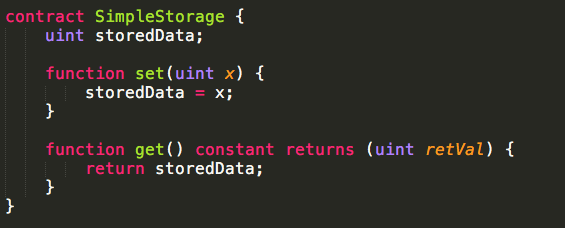
\includegraphics[width=1.4\textwidth]{Figures/Simplestorage}}
\decoRule
\caption[]{}
\label{fig:Simplestorage}
\end{figure}

\subsubsection{Dapps}
Dapp is short for distributed application. In the context of Ethereum a dapp is a complete application that incorporates not just a smart contract system (for executing something akin to server side logic) but also a client side user interface and any other architectural components. \\

Client side interfaces can be built with the same Javascript/HTML/CSS stack as normal web applications. It is common to see distributed filesystems such as IPFS (discussed in \ref{subsec:ipfs}) form part of dapp architectures. 

\subsubsection{Value Proposition}
The above description of Ethereum is fairly technical and esoteric. It is important to maintain sight of the purpose of such technology or, in the parlance of startup culture, the value proposition. The following question was raised at Ethereum DevCon1 during a panel on "The pathway to Ethereum adoption" \cite{devconvid}:\\

"I'm really excited about the potential of Ethereum to form the bedrock of a new socioeconomic paradigm. However, I'm not a developer, I'm not a dude, I don't work in bank, so I get the feeling you're baking a fatal flaw into this system at its inception by focusing on such a narrow demographic. What outreach plans do you have to encourage demand rather than focus on supply?".\\

The question highlights a misunderstanding about the value proposition of Ethereum. Unlike some other blockchain systems, such as Bitcoin, Ethereum is intended as a tool for application developers, not as a platform for end users. The offer to developers is a computation platform that is highly available, secure and transparent, has authentication and payment built in and is highly interoperable. However, performance requirements and costs also mean that Ethereum is not suitable for every application. 

\subsection{The InterPlanetary File System}
\label{subsec:ipfs}
The Inter Planetary File System (IPFS) is a content addressed, versioned, peer to peer file system. It aims to enable the creation of completely distributed applications and to make the web faster, safer, and more open.\\

IPFS synthesises the innovations behind many projects including the Self-Certifying File System\cite{mazieres1998escaping}, Kademlia\cite{maymounkov2002kademlia} (distributed hash table), BitTorrent and Git to propose a new alternative web protocol. The motivation and technical specification for IPFS has been well articulated by Benet in both the IPFS white paper\cite{benet2014ipfs} and a seminar at Stanford university\cite{IPFSVid}.

\subsubsection{The Problems}
In his Stanford seminar Benet highlights many challenges faced by the current web infrastructure:\\
\\
\keyword{Bandwidth}\\
The bandwidth of the network is not increasing at a significant rate. \\
\\
\keyword{Usage}\\
Storage prices are decreasing at a faster rate than the price of bandwidth. At the same time the demand for large data content is increasing e.g video conferencing, high definition media, 360 video etc. The combination leaves the impression that the network is actually slowing down.\\
\\
\keyword{Demand}\\
More and more devices and global populace are coming online. Extra demand is placing more strain on the network. Lesser economically developed countries experience the highest levels of network latency.\\
\\
\keyword{Centralisation}\\
Most of the data we use is controlled and maintained by a handful of organisations. This makes the data susceptible to physical disasters\cite{DCFire} as well as digital attacks. Furthermore, distribution of content is inefficient as the same data is sent across the network hundreds, thousands or even millions of times.\\
\\
\keyword{Permanence}\\
Content is addressed by location. The consequence is that if content is moved the link is broken and if the server is simply taken down the content may be lots forever.\\
\\
\keyword{Censorship}\\
The centralisation of services makes it very easy to censor communication and information applications by controlling the gateways for nation or state internet connections. Totally in browser applications using distributed data in peer to peer networks are resilient to weak links.\\
\\
\keyword{Resilience}\\
Whilst less severe than censorship, ISP outages and internet breakages are still a practical concern. The server client asymmetry makes it difficult for users to communicate and share data on a local area network when disconnected from the wider internet. \\
\\
\keyword{Control \& Security}\\
The transmission of data is typically secure but it is often stored in unencrypted formats both on the server and in the browser. \\

\subsubsection{The IPFS Solution}
\begin{figure}
\centering
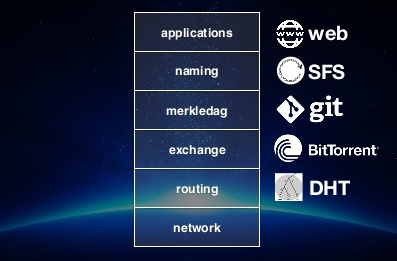
\includegraphics[width=\textwidth]{Figures/IpfsStack}
\decoRule
\caption[IPFS Stack]{The IPFS technology stack}
\label{fig:IpfsStack}
\end{figure}

Figure \ref{fig:IpfsStack} shows the various levels of, and contributions to, the IPFS stack. The core of IPFS is formed by the Merkle DAG (directed acylic graph). The IPFS Merkle DAG is a directed acyclic graph whose edges are merkle links. Essentially, this means that content can be addressed by a deterministic hash of the content itself i.e the root of a merkle tree structure. The use of merkledags, as with Git, also makes it possible to work offline first and version content. The properties that fall out from using Merkle DAG are that objects can be: a) retreived via their hash, b) integrity checked, c) linked to others and d) cached indefinitely. This all helps to make objects permanent. However, IPFS also implements a naming system, based on the work around self certifying file systems, that makes it possible to overlay the 'forest' of immutable objects with mutable links.\\ 

Distributed hash tables and block exchange peer to peer protocols build a sophisticated way to distribute and move the data (merkledags) as effectively as possible.

\section{Cooperative  Forms of Organisation}
\subsection{Brief History}
From the onset of  the industrial revolution a number cooperative and mutual responses emerged to the rapid growth of urbanisation, private companies and market mechanisms.  These include building societies, friendly societies, retail and wholesale cooperatives that aimed to provide services or benefits (access to housing, health care, out of work benefit, wholesome food etc) to defined communities of members.\\

\begin{figure}
\centering
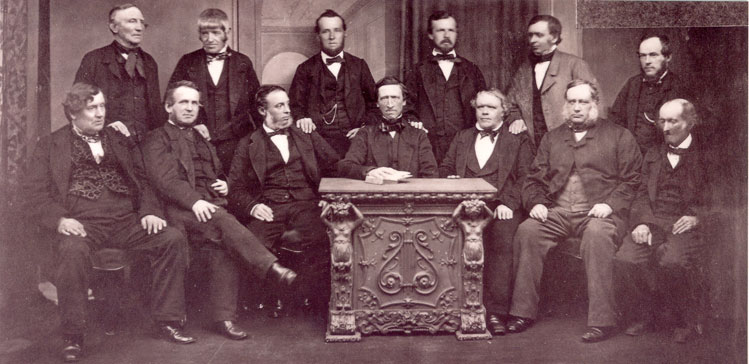
\includegraphics[width=\textwidth]{Figures/rochdale_pioneers}
\decoRule
\caption[Rochdale Pioneers]{The Rochdale Pioneers}
\label{fig:pioneers}
\end{figure}

The Rochdale Society of Equitable Pioneers, who formed in 1844\cite{Pioneers}, became the most successful and long lasting cooperative collective and are widely considered to be the founders of the modern cooperative movement. This is largely attributed to their documentation of cooperative principles\cite{Principles}, which established a values based organisational framework that subsequent cooperatives were able to adopt.\\

Throughout the rest of the century, many more cooperatives formed in the United Kingdom and independent movements also emerged elsewhere, such as credit unions in Germany and consumer cooperatives in the U.S.A. The colonial pursuits of European nations carried the cooperative model across the continents to India, Africa and South America where there remain strong cooperative communities to this day \cite{Coops_india_wiki}\cite{Coops_india}\cite{Kenya_coops}.\\   

In 1863, the Rochdale Pioneers merged with over 300 other cooperatives across Yorkshire and Lancashire to establish the North England Co-operative Society - which later became known as the CWS (Cooperative Wholesale Society). The CWS merged with more cooperatives throughout the 20th century and is recognisable on most UK high streets today as The Cooperative group.\\

\subsection{Principles Of Cooperation}
A brief summary of the seven principles of cooperation as defined by The International Cooperative Alliance\cite{ICA}, an adaption of the original principles defined by Rochdale Pioneers:\\

\begin{enumerate}
\item \keyword{Voluntary and Open Membership} \\ Co-operatives are voluntary organisations, open to all persons able to use their services and willing to accept the responsibilities of membership, without gender, social, racial, political or religious discrimination.

\item \keyword{Democratic Member Control} \\ Co-operatives are democratic organisations controlled by their members, who actively participate in setting their policies and making decisions. 

\item \keyword{Member Economic Participation} \\ Members contribute equitably to, and democratically control, the capital of their co-operative.

\item \keyword{Autonomy and Independence} \\ Co-operatives are autonomous, self-help organisations controlled by their members. Any terms always ensure the democratic control of the membership and maintain co-operative autonomy.

\item \keyword{Education, Training and Information} \\ Co-operatives provide education and training for their stakeholders and inform the general public - particularly young people and opinion leaders - about the nature and benefits of co-operation.

\item \keyword{Co-operation among Co-operatives} \\ Co-operatives serve their members most effectively and strengthen the co-operative movement by working together through local, national, regional and international structures.

\item \keyword{Concern for Community} \\ Co-operatives work for the sustainable development of their communities through policies approved by their members.

\end{enumerate}

\subsection{Scale}
A report carried out by CICOPA (The International Organisation of Industrial and Service Cooperatives) estimates that cooperatives employ almost 12\% of the entire working population of the G20 countries and that co-operative enterprises generate partial or full-time employment involving at least 250 million individuals worldwide, either in or within the scope of co-operatives \cite{roelants2014cooperatives}.\\

The UK cooperative sector turned over 37 Billion in 2015\cite{Cooperative_economy}. In Denmark consumer co-operatives in 2007 held 36.4\% of consumer retail market (source: Coop Norden AB Annual Report 2007). In Japan, the agricultural co-operatives report outputs of USD 90 billion with 91\% of all Japanese farmers in membership (Source: Co-op 2007 Facts \& Figures, Japanese Consumers' Co-operative Union.). In Malaysia, 6.78 million people or 27\% of the total population are members of co-operatives (Source: Ministry of Entrepreneur and Co-operative Development, Department of Co-operative Development, Malaysia, Statistics 31 December 2009).\\

The cooperative movement involves millions of people and contributes to significant portions of the economy worldwide.\\

\subsection{Cooperative Forms}
Although all coops unite under one banner there are a variety of cooperative forms depending on which group of stakeholders constitute the membership. The main types of cooperative forms include:\\\\
\keyword{Worker coops}\\
Employees of the business form the membership e.g Suma wholefoods\cite{Suma}.\\\\
\keyword{Consumer coops}\\
Members are consumers or customers who buy goods or services from their cooperative e.g The Cooperative group\cite{TheCoop}.\\\\
\keyword{Producer or Agricultural coops}\\
Many dairy farmers form producer coops. Members are producers who cooperate to make, market and sell their products.\\\\
\keyword{Multi stakeholder coops}\\
A hybrid form where multiple classes of membership coexist such as workers, producers and consumers.\\\\
\keyword{Housing coops}\\
Similar to a consumer coop. Members share ownership of residential property. \\


\subsection{Legal Incorporation \& Official Bodies}
Across the world cooperatives incorporate as legal entities in many different forms such as charities and limited companies. Whilst some countries, such as the UK, have legislation that legally acknowledge cooperative forms of organisation (The Co-operative and Community Benefit Societies Act 2014\cite{CoopAct}), many countries do not.\\

Although not always a legal requirement most cooperatives have a set of documents that outline their specific governance processes. Such documents are often required to register with official bodies, such as Co-operatives UK\cite{CoopsUK}. Measuring the commitment to the cooperative principles is somewhat subjective and these official bodies fulfil a role of authority on cooperative identity.

\subsection{The Cooperative Movement Today}
\keyword{The Cooperative group in the UK}\\
In 2014 the Cooperative Group, one of the largest cooperatives both in the UK and in the world, reported billions of pounds in losses. Former city minister Paul Myners was commissioned to run an independent investigation into the crisis and concluded that it was essentially caused by serious problems of incompetence, stemming from the group's governance structures. \\

The Co-op voted in favour of Myners proposed reforms in 2014 and more recently have appointed Mike Bracken, the former Government Chief Data Officer and Executive Director of Digital, who has been celebrated for bringing agile processes into government\cite{AgileGov}, as their new digital officer\cite{bracken}. It remains to be seen how the Cooperative group will develop under it's new structure and with it's new digital direction but it undoubtedly faces twin challenges of both maintaining cooperative organisation and developing member participation at scale.\\
\\
\keyword{Open coops}\\
There is an emergent notion of an 'open coop' that combines best practices from both the cooperative and open source movements\cite{OpenCoop}. Definitions of 'open coops' also specify a commitment to the organisation and co-production of the commons on a global basis (see ref). The requirement for these new cooperative definitions can be understood as a product of the web which is a) creating digital and tech coops who are naturally aligned with open source values and b) eroding the geographical and national boundaries previously limiting cooperative activity.\\
\\
\keyword{Platform Coops}\\
Another emergent notion is that of platform cooperatives\cite{PlatformCoop}. The case made by its proponents\cite{TreborPC} is that internet platforms (such as Uber, Airbnb, Taskrabbit etc), that form the basis of the 'sharing economy', are very good at sharing the risk (e.g cars, houses, maintenance, insurance), which is externalised to the platform users, but not very good at sharing the platform itself. The value creators for big Internet platforms (e.g drivers, hosts, cleaners, content creators) have little or no democratic voice and suffer by the extractive nature of the 'middleman' role played by the platform.\\

Whilst the benefits of platform based services are readily identified\cite{TreborPC} (rise of freelance work, building of real social networks, service over ownership, quality control or accountability through reputation systems) the argument is that the nature of employment is often precarious, undemocratic and insecure. \\

The proposed solution, is to takeover and rebuild platform services as cooperatives. Such platforms would provide all the same benefits but improve worker and stakeholder relationships.\\
 
The idea is growing in popularity. There are already a number of platform cooperatives forming (Fairmondo\cite{Fairmondo}, Resonate\cite{Resonate}) and many events and gatherings have been organised.\\

\section{Related Work}
\label{subsec:RelatedWork}
\subsection{Loomio}
Loomio\cite{Loomio} is a web application that assists groups with collective decision making processes. Loomio is a cooperative social enterprise that has been 'incubated' by the Enspiral network\cite{Enspiral-loomio}. Enspiral has been described as the best working example of an open cooperative\cite{Enspiral}.\\

\subsection{Boardroom}
\label{subsec:boardroom}
Boardroom is a decentralised governance application being developed on Ethereum that allows users to create organisational boards that can add or remove members, elect a chair, create subcommittees and allocate budgets. By using Ethereum, Boardroom adds a layer of security, auditability and transparency to help the governance processes of most traditional business architectures. Boardroom also takes advantage of the interoperability of the Ethereum ecosystem and has an extendable plugin architecture to facilitate the use of other Ethereum applications such as  crowdfunders, prediction markets etc.\\

\subsection{DigixDAO and The DAO}
\label{subsec:DAOs}
DAO stands for decentralised autonomous organisation. There has been a lot of speculation about the propensity of the Ethereum platform to host DAOs as well as how successful such projects might be. According to Vitalik Buterin, creator of the Ethereum platform, a DAO "is an entity that lives on the internet and exists autonomously, but also heavily relies on hiring individuals to perform certain tasks that the automaton itself cannot do."\cite{DAOBlog} DAOs have internal capital that it is able to spend and use to reward certain activities. \\ 

This year saw the launch of two DAOs on Ethereum. The DigixDAO\cite{Digix}, a platform for trading gold backed tokens, reached it's goal of \$5.5 million in under 12 hours in March\cite{DigixCrowd}. TheDAO\cite{TheDAO}, which is essentially a public investment fund where members can vote on proposals and subcontract work, is estimated to have raised over \$120 million in May which would make it the most successful crowd fund ever\cite{DAOCrowd}.\\

Given the arrival of DAOs, it is interesting to consider the concept of a Decentralised Autonomous Cooperative.\\

\subsection{Robin Hood Asset Management}
\label{subsec:RobinHood}
The Robin Hood Coop (RHC)\cite{RHC} are a hedge fund organised as a cooperative. Compared to the majority of other hedge funds the RHC operates at 'ridiculously' low costs and uses a 'parasite' algorithm that copies the behaviour of the most successful traders on the market. The profit generated by RHC investments is invested into projects that are building 'the commons'. \\

In their April newsletter, RHC announced the launch of a new innovation "a share \& member management system on the Ethereum blockchain". The newsletter is scant on details but the acknowledgment of Ethereum's potential utility by cooperative enterprises is a welcome validation of this study. 

\subsection{BuyCo.io}
\label{subsec:buyco}
BuyCo.io is a 'collaborative purchasing toolkit' that aims to leverage blockchain technology to make it easier for businesses and individuals to join together and form buying or purchase cooperatives. "Traditionally, buying cooperatives are time and labour intensive to set up and run. BuyCo.io allows you to set one up in seconds with ordering, supplier management, governance, escrow and payment processing all fully automated."\cite{BuyCo} Buyco claim that by using blockchain technology they are able to provide greater levels of user control and faster transaction times at much lower costs than traditional e-commerce platforms. The project is currently in the proof of concept stage. The BuyCo whitepaper can be found on their website (see ref). \\

Both BuyCo and the Robin Hood Coop are likely to face similar design and implementation challenges to those explored in this study. Future work in this area would benefit from the input of these projects and collaboration between the many emerging cooperative based approaches to blockchain technology.



 
% Chapter 1

\chapter{Research And Design} % Main chapter title

\label{ResearchAndDesign} % For referencing the chapter elsewhere, use \ref{ResearchAndDesign} 

\section{Cooperative Governance}
\label{subsec:CooperativeGovernance}
The objective of this section is to outline the current processes surrounding cooperative governance, identify points of friction that are likely to arise as these processes are scaled and finally, to propose ways an Ethereum based application could provide solutions.

\subsection{Current Governance Model}
The best points of reference for understanding the current governance model of co-operatives are governing documents. Every cooperative has a set of governing documents which lay out the constitution and bylaws of the organisation. They are important in ensuring the overall direction, supervision and accountability of the cooperative. In plain terms governing documents help to establish: what the coop will do, who will do it and how they will do it. \\

The main topics covered in a set of governing documents are: membership, democracy, voting, general meetings, dissolution, administration, application of profits and dispute resolution. Because many cooperatives have similar governance requirements and take on a similar form, size and/or sector, there are a number of 'model rules' available to startup coops. For example, the trade organisation, Cooperatives UK \cite{modelRules} and Somerset Cooperative Services\cite{somersetRules} (SCS) both provide sets of model rules. The following subsections describe the main elements of cooperative governance as commonly defined within governing documents.\\

\subsubsection{Membership}
Co-operatives traditionally have been established to serve the specific interests or needs of a certain class of stakeholders, such as workers or consumers, however, each membership group has a different relationship to the cooperative entity. The first principle of cooperation, "voluntary and open membership", is interpreted within this context. A worker cooperative (for example, Suma\cite{Suma} with some 200 members) whilst having an open, non-discriminatory membership policy will also have a set of selection and appointment criteria for employees who wish to become members.  A consumer cooperative (such as, The Cooperative\cite{TheCoop}, 7m members) will have much less restrictive membership conditions: most individuals can become stakeholders by filling out a form and shopping at the group's stores.  A recent development has been the creation of Multi-stakeholder Cooperatives (MSC) that opens up membership to different classes of stakeholder: workers, consumers, users, investors etc through the use of the SCS's Somerset Rules.\\

Beyond defining stakeholder boundaries most governing documents also specify a minimum age for members (usually sixteen), a fee or minimum share purchase, the value of shares any member may hold, member commitments to governance and conditions for member termination.\\

\begin{figure}
\centering
\makebox[\textwidth][c]{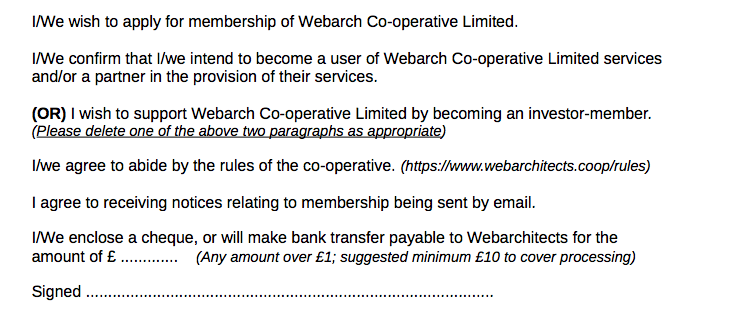
\includegraphics[width=1.4\textwidth]{Figures/webarchForm}}
\decoRule
\caption[]{A section of a membership application form for Webarchitects multi stakeholder cooperative illustrating example conditions of membership}
\label{fig:webarchForm}
\end{figure} 
Figure \ref{fig:webarchForm} is an extract from the membership application form for Webrarchitects\cite{webarchitects} (a multi stakeholder co-operative). Besides providing general personal information such as name, email and address, prospective members must also sign up to rules or conditions of membership.\\

\subsubsection{General Meetings}
General meetings (GMs) are the 'sovereign body' of a cooperative. Although any member may propose a resolution at a GM, the main focus is normally the election of directors and/or deciding on the application of profits. Co-operatives have a main annual general meeting (AGM) as well as several other general meetings throughout the year. Figure \ref{fig:workerCoopGM} shows an extract from the Coops UK Worker Co-operative Model.\\
\begin{figure}
\centering
\makebox[\textwidth][c]{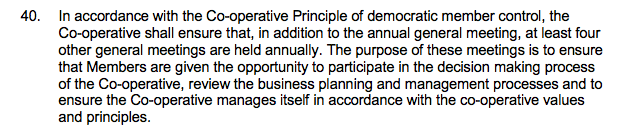
\includegraphics[width=1.4\textwidth]{Figures/WorkerModelGM}}
\decoRule
\caption[]{A section of the Coops UK worker co-operative model rules outlining the purpose of general meetings}
\label{fig:workerCoopGM}
\end{figure} 

General meetings may be called at the discretion of the board of directors or following a demand from a set threshold of the membership. For example, the worker co-op specifies the lesser of one tenth of or 100 members.

\subsubsection{Board of Directors}
A board of directors is a subset of the membership in large co-operatives, appointed to manage the business of the cooperative and who typically have the right to exercise any powers that might be exercised by the cooperative as a whole. It is important for the survival of the co-operative that directors have sufficient competence to effectively and efficiently manage the business. Some co-operatives pass standing orders to define the necessary skills and qualifications for director positions.

\subsubsection{Voting}
\begin{figure}
\centering
\makebox[\textwidth][c]{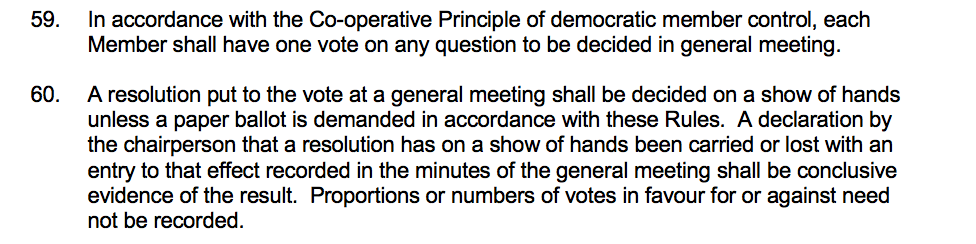
\includegraphics[width=1.4\textwidth]{Figures/WorkerRulesVoting}}
\decoRule
\caption[]{A section of the Coops UK worker coop model rules illustrating an example voting process.}
\label{fig:WorkerRulesVoting}
\end{figure} 
Co-operatives are almost always 'one member one vote'. The voting process in small cooperatives may just be a show of hands. Large member coops must have sophisticated member engagement strategies to inform, encourage and enable members to take part in postal or online ballots to elect directors or pass important motions. Figure \ref{fig:WorkerRulesVoting} shows the main voting clauses from the Coops UK worker co-operative model rules. Voting in multi stakeholder cooperatives can be slightly more interesting as the rules must protect against unfair representation or dominance of a single stakeholder group. Figure \ref{fig:SomersetVoting} shows an extract from the Somerset Rules. The Somerset rules also specify that no resolution may change the rules on class weighting themselves. 
\begin{figure}
\centering
\makebox[\textwidth][c]{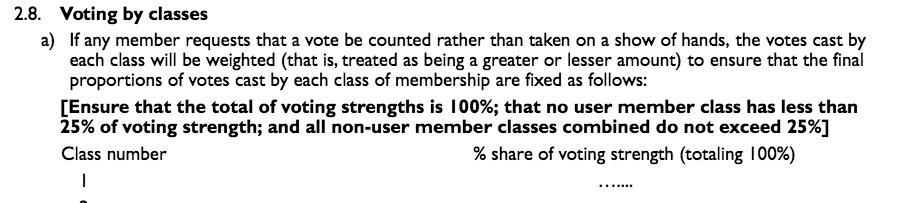
\includegraphics[width=1.4\textwidth]{Figures/SomersetVoting}}
\decoRule
\caption[]{A section of the Somerset multi stakeholder model rules illustrating the complex and contractual nature of class based voting.}
\label{fig:SomersetVoting}
\end{figure} 

\subsubsection{Quorum}
A quorum simply defines the minimum number of members that must be present at decision making meetings in order to carry out business. Its purpose, like that of voting thresholds (such as, "two thirds majority") for changes to key parts of the constitution, is to safeguard the organisation from control or dominance by unrepresentative groups or decisions.

\subsubsection{Resolutions}
A resolution or motion is a formal proposal to change some aspect of the organisation's behaviour or practice. High level decision making works through proposing and voting on resolutions. Normally governing documents make a distinction between normal and extraordinary resolutions and the proportion of the vote required to pass the resolution. Normal resolutions are typically non-constitutional and require a lower majority. Extraordinary resolutions are often constitutional and propose changes to the rules of the cooperative itself. Some co-operatives choose consensus decision making and require 100\% agreement on all resolutions.

\subsection{A Scalable Governance Solution}
For most co-operatives, the tried and tested governance models described above are very effective. The problem which has been identified in the motivation to this study, however, is that when scaled, they become less efficient and less effective at representing the membership: barriers are created by membership numbers, spatial distribution and time -  to attend meetings and/or understand the issue.  The systems put in place to overcome these problems traditionally have been "representative" based branch and regional meetings, postal and online balloting, all of which create considerable friction to membership participation. This is illustrated by The Cooperative group where, despite the Mynors led overhaul\cite{Myners} of the governance architecture, low participation remains problematic as the Interim Results of the Group, 4, July, 2015 conclude:\\

"The fledgling nature of the new democratic structures was reflected in voter turnout at the AGM, with  3\% of eligible members casting their votes. Our ambition is to see this number substantially increase as we implement our member engagement programme, which will launch in mid-2016. This aims to reverse many years of declining member participation."\cite{CoopParticipation}\\

The following subsections describe how an Ethereum based application might address scaling issues faced by the various elements of governance.\\

\subsubsection{Membership}
Large co-operatives store membership details and attributes in databases. These provide the basis on which the organisation carries out "member relationship management" functions, more typically termed customer relationship management, that is, enroll and validate membership identity and credentials, carry out communications, store transaction details, surveys and conduct postal or online ballots etc.  The creation, storage, configuration and use of this data must comply with UK law as set out in the Data Protection Act\cite{DataProtection}: 
\begin{itemize}
\item used fairly and lawfully
\item used for limited, specifically stated purposes
\item used in a way that is adequate, relevant and not excessive
\item accurate
\item kept for no longer than is absolutely necessary
\item handled according to people's data protection rights
\item kept safe and secure
\item not transferred outside the European Economic Area without adequate protection
\end{itemize}

The data holder in this instance must have considerable organisational competence to manage this information. A trusted relationship emerges between the members and the data holder, in this case an organisation over which the members have democratic control and scrutiny.\\

There are a number of ways the Ethereum platform can aid the legal compliance of a governance application:
\begin{itemize}
\item Public private key authentication means that access to data can be restricted to only permissioned key holders. This offers a much higher level of cryptographic security than many existing systems. Encryption of data on the blockchain is discussed further in section \ref{sec:blockchainprivacy}.
\item Member information does not need to be held by every individual co-operative. It can be stored in the blockchain once where it is controlled by its owner. This makes it much easier to keep data accurate and secure.
\item The resilience and high availability of the peer to peer network mean data is safe from damage or disaster.
\end{itemize}

Further to this, Ethereum's corruption resistant nature and the transparency of contract code mean a governance application can establish a high level of trust with members. Members can be uniquely identified by an Ethereum account (discussed further in section \ref{sec:identity}) which makes it easy to collect membership fees in Ether and enforce secure voting.\\

\subsubsection{General Meetings}
General meetings create practical spatial and temporal barriers to member participation - people have to make a considerable effort to be in the right place at the right time to engage in the discussion and the decisions, this naturally discriminates against anyone who is unable to travel or cannot attend at a particular time.  When coops are small, localised or workplace based this is not a significant issue.  When coops are large and/or distributed general meetings tend to become representative of the members who have the time and resources etc to take part. Location, distance, time, cost etc increase barriers to participation. General meetings to some extent could be characterised as an artifact of the pre-web era but despite the widespread adoption of digital decision making tools, such as Loomio (see \ref{subsec:RelatedWork}), they still form a central pillar of co-operative governance. There are a number of possible reasons for the "live" F2F (face to face) GM's popularity, including: the quality of the abstracted online communication - loss of immediacy; lack of technical competency to set up digital systems and lack of trust in the security and auditability of these tools. \\

The business - structured list (agenda) of decisions to be taken - at a General Meeting typically will comprise:
\begin{itemize}
\item documentation with a valid and verifiable origin within the organisation, that is, put forward by a legitimate body or members according to the standing orders,
\item a deliberative process where arguments for the proposal are set out and discussed, amendments can be made and the final wording of the motion put to a vote or poll.
\end{itemize}

There are three key aspects to this process:\\

Firstly, the ability of the participants to "be in the room", have sight of the proposal, see and hear the deliberations, have the opportunity to speak or suggest amendments.  \\

Secondly, the documentation of a resolution and the final form must be accurately configured to reflect the amendments (transactions) to be put to the vote, and \\

Thirdly, the rules or standing orders must be understood and followed by either the live or the digitally enable processes.\\

A range of applications may be used to overcome the spatial and temporal barriers and recreate the real world experience and processes used in GMs, for example, streaming video and audio (citrix), text based exchanges (Loomio) and possibly in the future Virtual Reality Headsets, if these become widely available. The role of an Ethereum application would be to deal with configuration management - recording and tracking changes (versions of the proposal), establishing the final form of words that will be put to the vote and the voting process itself (following appropriate rules defined by a co-operatives standing orders). Such an application would offer similar functionality to tools such as Loomio but with security guarantees that make it usable for binding decisions. \\

An Ethereum based application could therefore fulfill the requirements of the decision making process currently facilitated by GMs whilst simultaneously offering a high enough level of trust and security to enable its adoption. Costs could be reduced whilst participation and efficiency are increased. The ability to make decisions collectively is no longer restricted by the logistical constraints of organising physical real world meetings.\\

\subsubsection{Resolutions}
Proposals or resolutions must be documented and be capable of dynamically changing in response to amendments in a General Meeting scenario. An Ethereum application could enable digital collaboration whilst permanently versioning changes to proposals into the blockchain. A smart contract system could trivially render a final form immutable and make it available to everyone with valid voting credentials. In addition, many constitutional or extraordinary resolutions passed by a co-operative could be implemented by the smart contract system itself. For example, the normal resolution level of a co-operative must be stored in the smart contract system in order to implement a correct voting algorithm. Executing a proposal that changes the normal resolution would therefore be as simple as changing a variable within a program!\\

\subsubsection{Voting}
At the point of voting on a proposal it is necessary to accurately record that valid votes are cast, that is, by members entitled to vote, that a result of the vote is accurately recorded and can be audited should that be required.  Clearly counting hands doesn't scale, neither is it private or easily verifiable and is subject to the human error of the "tellers". Paper based ballots and postal voting where the whole membership is required to vote can scale, but become costly, unwieldy, slow as well as creating friction to participation.  The prospect of electoral fraud may be of less significance in organisational ballots where there is little to be gained personally by individuals but any system should be sufficiently robust that fraud is guarded against.\\

A voting system based on Ethereum has the potential, through the use of smart contracts using transactions signed with verified public-private keys, to digitally enable whole member votes to be deployed securely and rapidly across a widely distributed membership. This does depend on members being willing to use the internet and the distributed applications. Many of the voting rules, such as those shown in figure \ref{fig:SomersetVoting}, lend themselves naturally to the kind of logic that can be embedded in a smart contract system. \\

\subsubsection{Quorum and Thresholds}
Quorum and thresholds can be designed into smart contract systems to ensure the vote is valid in accordance with agreed rules. The system can be designed to automatically "defeat" or pass any resolution that does not reach the threshold at the closing date.\\

\subsubsection{Boards}
Unlike general meetings, the existence of directors is less a product of available technology and more concerned with efficient operation. Not all decisions need to be taken at the level of the cooperative, that is, by the full membership or General Meeting. Even within large distributed cooperatives directors will be required to manage operational matters. \\


\section{Privacy on The Blockchain}
\label{sec:blockchainprivacy}
Ethereum is a permissionless blockchain. This means any peer can freely join the network and participate in the mining process. The security of Ethereum is reliant on the ability of any of these peers to validate the correct linking of, and state transitions between, all blocks in the history of the chain. This group consensus is what makes blockchains so valuable but it is also the reason why the whole blockchain must be publicly visible (at least to the permissioned set of peers). If it were possible to censor parts of the chain or hide certain transactions then the validation process would break down and all trust in the network would be lost. In Ethereum this means any call to contract code, any change in contract state or any transfer of ether is transparent. This is a fairly obvious point but worth making because it is easy to lose sight of the basic when dealing with the complex.\\

The transparency of the Ethereum blockchain introduces a couple of obstacles for application developers. The first one is how private data should be managed. The second, and slightly more complex, is how computations that require the input of private data can be executed. This section introduces some possible approaches to tackling these issues both of which are relevant to the development of Go-op. \\

\subsection{Storing Private Data}
As discussed in \ref{subsec:CooperativeGovernance} , a likely requirement of Go-op is the protected storage of membership information. Cooperative members should have access to the personal information of other members but such information should not generally be accessible to any other party. \\

Private data can be stored on a blockchain by simply encrypting it first. The ciphertext will be publicly visible but the information will be hidden. An Ethereum account address is derived from the public key of a public-private key pair generated using ECC (Elliptic Curve Cryptography) and the SECP-256k1 curve parameters (described in the Yellow Paper \cite{Yellowpaper}). Taking advantage of these key pairs, encryption of member information could potentially be achieved as follows:\\

For each intended recipient of the data:\\
\begin{enumerate}
\item Retrieve a public key from their public address. Possible using the Solidity ecrecover function\cite{SolidityCheatsheet} or in the browser (manually\cite{StackExchangeAddress} or using a library\cite{WalletJS}).

\item Use the public key to encrypt the data in the browser using ECC asymmetric encryption.

\item Store the ciphertext in the Ethereum blockchain.

\item Recipients read from blockchain and decrypt using their private key (obtainable from their address following similar process step 1) 

\end{enumerate}

A nice aspect of this approach is that it doesn't introduce any additional key management complexity and by taking advantage of the 'Web3.0 architecture?'(see \ref{sec:web3Arch}) the process can also be simplified somewhat. The ciphertext can actually be stored in a distributed file system (such as IPFS see  \ref{subsec:ipfs}) and a link (e.g ipfs hash) can be stored in the blockchain instead. \\

Asymmetric encryption techniques such as ECC however, are fairly computationally intensive which could make this approach unwieldy in the face of thousands of users. More importantly, asymmetric encryption schemes are not generally recommended for encrypting large messages and are instead used for the secure exchange of symmetric keys. This form of hybrid approach is thought to be more secure and efficient. For encryption on Ethereum, such a process might look like the following:

\begin{enumerate}
\item Generate a symmetric key. 
\item Encrypt data with symmetric key (e.g using AES).
\item Store the encrypted data (or IPFS address of encrypted data) in the blockchain.
\item For each intended recipient, encrypt the symmetric key following an asymmetric encryption method similar to the one described previously.
\item Store mapping of Ethereum accounts to matching ciphertexts of the symmetric key on the Ethereum blockchain (again this can be more efficiently stored in IPFS and referenced from blockchain)
\item Recipients read from blockchain to find a) the ciphertext of the data (step 3) and b) the ciphertext of the symmetric key (step 5)
\item Recipient decrypts the symmetric key using their private key and then decrypts the data using the symmetric key.
\end{enumerate}

This method still requires the same number of asymmetric encryption operations as before but the process is less computationally intensive because the size of the plaintext (i.e the symmetric key) encrypted in this way is constant and much smaller. The encryption of any potentially large amounts of data only needs to be performed once using symmetric encryption.\\

Any change to the encrypted information is relatively easy to handle because, providing a suitable block cipher mode is chosen, the same symmetric key can be reused. Granting access to new accounts is also easy because it only requires one additional encryption of the symmetric key with the public key of the new account. The drawback is that whenever a key needs to be revoked, the symmetric key is compromised and any future encryption would need to repeat the whole process with a new symmetric key. From a security perspective, we must assume that any information encrypted with the old symmetric key is known to the excluded party, it is not possible to enforce forgetfulness. \\

Controlled access to information and privacy in general are common requirements for many applications. It is probable that, as the Ethereum ecosystem matures, more tools and solutions will become available to make this process easier and safer for application developers. \\

\subsection{Computing Private Data}
A more complex requirement than the storage of private information is performing computation with it. Consider anonymous voting, which is highly relevant to the Go-op application, where the objective is to calculate the outcome of a vote without revealing any information about the choices of individual participants. Calculating the result of a vote on Ethereum would make the process secure but, again, because execution of contract code is transparent, it makes it difficult to ensure privacy. A potential solution would combine some method of blinding a vote with a method for counting the blinded values.\\

Provable honest voting systems that protect voter privacy have been widely discussed\cite{PrivacyBlockchain}\cite{HonestElection}. Possible solutions include the use of ring signatures\cite{liu2004linkable}\cite{tsang2005short} and addition through homomorphic encryption\cite{HomoEncryption}.\\

\subsection{A Word on Solidity Access Modifiers}
Whilst the Ethereum blockchain is transparent, the Solidity language features various visibilities for functions and state variables (see Figure \ref{fig:AccessModifiers}, so what does this mean? \\
\begin{figure}
\centering
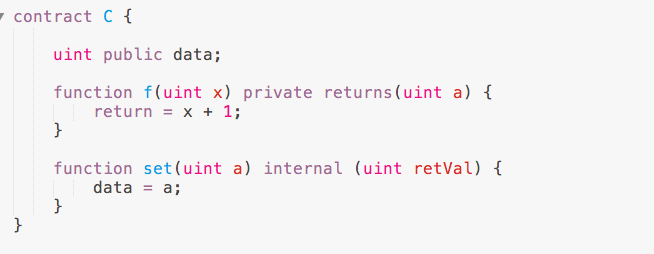
\includegraphics[width=\textwidth]{Figures/AccessModifiers}
\decoRule
\caption[]{}
\label{fig:AccessModifiers}
\end{figure}
Access modifiers within Solidity, like in many other languages, are designed to aid code encapsulation. Whilst they restrict the behaviour of executing contract code, and therefore help to catch bugs and errors at compile time, they don't provide any access modification to any external entity reading from the blockchain.\\

%%%%%%%%%%%%%%%%%%%%%%%%%%%%%%%%%%%%%%%%%%%%%%%%%%%
%%%%%%%%%%%%%%%%%%%%%%%%%%%%%%%%%%%%%%%%%%%%%%%%%%%
\section{Oracles And Identity Management}
\label{sec:identity}
For many real world and digital services the 'proof of identity' or KYC (know your customer) problem is very important. For financial service providers, knowing the customer can help to mitigate risk (issuing loans etc), avoid money laundering or protect against fraud. In any kind of democracy application such as Go-op, where we need to enforce the principle of 'one member one vote', identity management is key to fair representation and the avoidance of double votes.\\

The 'proof of identity' problem does not disappear when we move to the blockchain. Given that any Ethereum user can generate multiple accounts it is very tricky to identify an individual in a completely 'trustless' fashion. 

\subsection{e-Residency}
e-Residency is a transnational digital identity offered by the government of Estonia to any global citizen wishing to administer a location independent business online \cite{e-Residency}. To become an e-Resident applications must provide a photo ID and a copy of their pre-existing government issued identity (such as a passport). A background check is then conducted by Estonian officials before the applicant is able to collect the card, in person, to verify their identity. In return, e-Residents receive a smart ID card with a unique public private key pair that both proves the identity of a person and allows them to easily create digital signatures. Technically, digital certificate chains are used to prove that the key-pair within the e-Resident card are derived from a key-pair controlled by the Estonian government. \\

\begin{figure}
\centering
\includegraphics[width=\textwidth]{Figures/e-Residency}
\decoRule
\caption[]{}
\label{fig:e-Residency}
\end{figure}

Returning to the 'proof of identity' problem on Ethereum, e-Residency provides a way for the Estonian government to become the trusted authority on the identity behind an Ethereum account (see \cite{IDBereg} \cite{BertaniKYC} for more on this idea) but there are still a few barriers to practical implementation. Firstly, e-Resident cards use RSA encryption. Verification of RSA signatures 'on-chain' is not yet possible although this could well change in the future \cite{RSARequest}. Secondly, the Estonian government would need to engage with Ethereum and publish their top level certificates to the blockchain so that other contracts can use them for signature verification. Given their commitment to e-Residency and history in pioneering technical solutions\cite{EstoniaE-Voting}, this doesn't seem too improbable. A temporary work around could be the use of a trusted 'oracle'\cite{BertaniOracles}, such as Oraclize\cite{Oraclise}.

\subsection{Curators}
TheDAO (briefly explained in \ref{subsec:DAOs}) is an Ethereum based organisation that is able to subcontract work to external, real world entities. Proposals for work are submitted to TheDAO as smart contracts and members vote to accept them. However, without knowing the identity of contract proposers, members have no idea whether proposals are legitimate, and therefore likely to be completed, or just spam. In general, the operation of TheDAO will be more efficient if the identity of service providers is known.\\
 
To solve this identity problem TheDAO introduces the concept of a 'curator'\cite{TaulCurators}. One of the main roles of a curator is to validate that any contractor who makes a proposal is a real person or organisation. This is an off the chain process that requires TheDAO members to trust the curators. Members of TheDAO can, at any time, vote to replace curators but the requirement for a trusted third party still remains.\\

This is a more localised approach to trust than e-Residency. The e-Residency card has the potential to form a general identity provision infrastructure that could be used by any Ethereum service. Managing identity this way would require all users of your application to be e-Residents. In contrast, the approach taken by TheDAO simply requires the election of a trusted member to validate identities 'off-chain' but any identification here is unlikely to pass muster within other organisations. \\


%%%%%%%%%%%%%%%%%%%%%%%%%%%%%%%%%%%%%%%%%%%%%%%%%%%
%%%%%%%%%%%%%%%%%%%%%%%%%%%%%%%%%%%%%%%%%%%%%%%%%%%

\section{Blockchain Time}
\label{sec:blocktime}
There are a couple of interesting design challenges surrounding smart contract applications that need to work with time. Firstly, how can accurate and reliable time measurements be accessed within the blockchain? Secondly, how can contract code react to an event at a specific time? For a governance or democracy application measuring time is important for closing ballots at the correct date. Ideally we would like an accurate notion of time (to make things as fair as possible) that we can react to in order to prevent further voting and to calculate the result.\\

\subsection{Accurate Timestamps}
For a block to be accepted by a miner, the state transition function has to produce the same output as it did for the block creator. If smart contract code used the host machine's (i.e miners) system time for its logic then this could easily \keyword{not} be the case because blocks are not created and validated at the same time. The only time reference that can be used, because it is consistent, is the timestamp of the block a transaction is included in. Ethereum smart contracts written in Solidity can access this time easily through the \code{block.timestamp} property. The problem with the block timestamp however, is that it is not necessarily accurate. The Ethereum protocol places some restrictions on timestamps but cannot be too strict because is must accommodate for drift in clocks across the network. Whilst this may be a cause for concern in highly time critical applications, in reality, the block timestamp is probably accurate enough for most usages.\\

\subsection{Scheduled Execution}
Unfortunately, because smart contract code can only be executed as the result of an external transaction and cannot simply 'wake up', the ability of contracts to schedule execution or react to time based events is limited. There are two possible solutions for smart contracts that need to execute code based on the time - eager and lazy evaluation. \\

A contract working eagerly will somehow arrange for an external transaction to call its evaluation code at a specific time in the future. In contrast, a contract working lazily will just wait for a transaction to occur 'naturally' and then, if the time of an event has passed, evaluate it's logic.\\
\begin{figure}
\centering

\includegraphics[width=\textwidth]{Figures/lazy}
\decoRule
\caption[]{Timeline of ballot contract calls with ;azy evaluation}
\label{fig:lazy}
\end{figure}
Figure \ref{fig:lazy} shows an example time frame for a ballot contract. When the ballot closes the contract may need to perform some additional logic to calculate a result or close the voting. Following a lazy approach, this is triggered by the 'read result' transaction which is the next transaction to occur. There are a couple of issues with the approach. Firstly, if no transactions 'naturally' occur after the ballot closes then the evaluation simply can't happen. Secondly, the 'read result' method must become a transaction because it might trigger evaluation code which updates state in the blockchain. Ideally, getting the result should just be a call and the first user to ask for it shouldn't have to pay!\\

To address these problems an 'eager evaluation' solution has been developed by the Ethereum community called the Ethereum Alarm Clock. For a small fee, the Ethereum Alarm Clock service allows contracts to schedule calls by registering their address and the definition of a function they would like to be executed. The Ethereum Alarm Clock service uses this payment to offer a bounty to any user account that makes the transaction at the scheduled time. The service creates a marketplace for function calls that any Ethereum user can participate in. Figure \ref{fig:eager} shows how a ballot would be closed using the Alarm Clock service.\\

\begin{figure}
\centering

\includegraphics[width=\textwidth]{Figures/eager}
\decoRule
\caption[]{Timeline of ballot contract calls with eager evaluation}
\label{fig:eager}
\end{figure}
The eager evaluation solution also has its flaws. Firstly, calls are scheduled for a given period of blocks into the future and not at a given time. Secondly, the service cannot guarantee that a call will be executed. It relies on an open market of rational actors but if no one wants to collect the fee for your function call then it cannot happen.\\

%%%%%%%%%%%%%%%%%%%%%%%%%%%%%%%%%%%%%%%%%%%%%%%%%%%
%%%%%%%%%%%%%%%%%%%%%%%%%%%%%%%%%%%%%%%%%%%%%%%%%%%
\section{Idealised Web3.0 Architecture}
\label{sec:web3Arch}
Dr Gavin Wood, author of the Ethereum yellow paper\cite{Yellowpaper} and lead developer of the c++ client, gave a talk at a Meetup in 2014 called 'The Ethereum Experience' (video\cite{Web3Vid} and slides\cite{Web3Slides} available) in which he outlined an idealised architecture for Web3.0 applications. In addition to Ethereum, Wood presents two complementary technologies (also developed by the Ethereum foundation) called Whisper and Swarm.\\ 

Swarm is a distributed file system that is very similar in nature to IPFS (see \ref{subsec:ipfs})\\

Whisper is a private and public messaging system built into Ethereum. Conceptually it is something akin to UDP (User Datagram Protocol) and enables dapps to communicate through instant transient messaging. Whisper uses probabilistic routing, high levels of encryption and is subscription based, meaning messages can easily be filtered.\\

Together, Ethereum, Swarm and Whisper form a complementary stack of tools for building completely distributed web applications.\\ 
\begin{figure}
\centering
\includegraphics[width=\textwidth]{Figures/DappArch}
\decoRule
\caption[]{}
\label{fig:DappArch}
\end{figure}

Figure \ref{fig:DappArch} is a conceptual diagram showing the interaction of three dapps in an idealised Web3.0 architecture. The green circles represent client computers, perhaps even a single program such as the Mist browser. The 'backend' of the dapp consists of logic split between javascript running in in the browser and the Ethereum blockchain. Dapps communicate dynamically using Whisper for public and private instant messaging and Swarm for file or content storage.\\
\begin{figure}
\centering
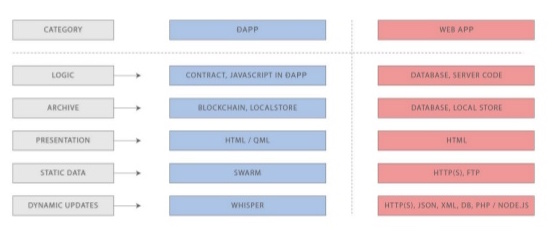
\includegraphics[width=\textwidth]{Figures/DappVWeb}
\decoRule
\caption[]{}
\label{fig:DappVWeb}
\end{figure}
\\
The process for loading a dapp in this system might go something like the following:\\
\begin{enumerate}
\item User opens their Web3.0 enabled browser such as Mist.
\item User searches for app in navigation bar e.g eth://go-op
\item A top level DNS contract in Ethereum returns address of static files for Go-Op front end within a distributed file system such as IPFS.
\item Mist browser fetches web app from distributed file system and renders it.
\end{enumerate}

\subsection{Status}
This is an idealised architecture because its components do not yet fully exist. Ethereum is currently at 'Homestead', one of the several milestones in a security led release process\cite{VinayLaunch} (we are still waiting for official release of Mist and Casper proof of stake protocol for example). According to Victor Tron (Ethereum core developer), both the go and c++ Ethereum clients have fully functional Whisper implementations\cite{TronStack}. However, other than a short section in the Web3 API, Whisper is not widely documented and at this point hardly appears in any community or official documentation.\\

Swarm is still under development by the Ethereum go team. At the time of writing they are working closely with IPFS to try and integrate the two projects\cite{DevUpdate}. \\

%%%%%%%%%%%%%%%%%%%%%%%%%%%%%%%%%%%%%%%%%%%%%%%%%%%
%%%%%%%%%%%%%%%%%%%%%%%%%%%%%%%%%%%%%%%%%%%%%%%%%%%
\section{Smart Contract Design Patterns}
\label{sec:scDesign}
Smart contract backends for distributed applications are typically composed of multiple components - "Every non-trivial DApp will require more than one contract to work well. There is no way to write a secure and scalable smart contract back-end without distributing the data and logic over multiple contracts."\cite{FiveTypes}\\

Although smart contracts might be thought of in a similar way to normal web services (they provide a public facing API at a specific address over a network) there are many differences that make the process challenging and demand special attention. \\

The first of these is the immutability of contract code. The code of an Ethereum contract account cannot be changed and is therefore bound to the account address. This implies that if we want to evolve smart contract systems over time we either have to redeploy them or design them in a highly modular fashion. Modular systems are generally the prefered option because it minimises costs, prevents blockchain bloating and maintains the same access address for service consumers. \\

Another challenge for smart contract systems is permission management. Ethereum applications are generally required to be secure. If a system grows into multiple contracts then besides modularity, contracts need to know who is calling them and what level of permissions they have. \\

This section introduces a couple of useful patterns to aid smart contract development.\\

\subsection{Events}
\label{subsec:events}
Front end dapp code uses the web3.js library\cite{Web3JS}, which exposes the Web3 Javascript API\cite{JavascriptAPI}, to interact with smart contracts. in turn, the web3 library communicates with the local Ethereum node through an RPC (Remote Procedure Call) interface. Depending on whether smart contract code modifies the blockchain (i.e changes contract storage state) a function call will either be a 'transaction' or a 'call'. Calls do not require gas to execute and a web3.js callback will be passed the same return value as the solidity function. Transactions however, need to be processed by the network. They require gas to execute and the argument passed to the callback is a transaction hash, not the return value of the solidity function. Return values for non-constant (state changing) contract functions are only returnable to calls from other contracts within the EVM not from an external call. A potential implication of this is that it becomes difficult for a dapp to know whether a transaction (i.e state changing function call) successfully completed or whether it failed (conditions, exceptions, out of gas etc). A simple design pattern that uses Ethereum events is used to handle this. \\
\begin{figure}
\centering
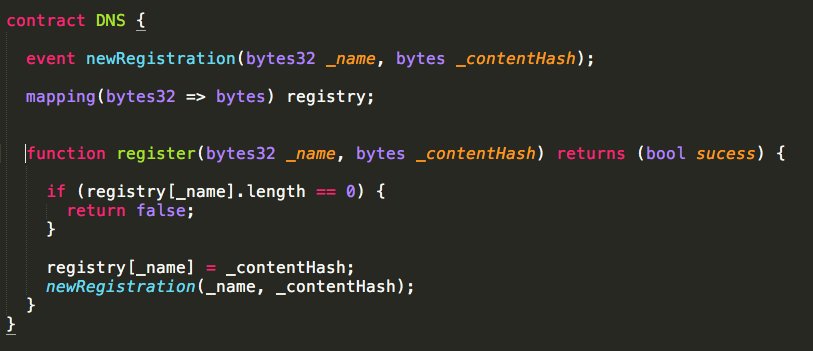
\includegraphics[width=\textwidth]{Figures/DNSContract}
\decoRule
\caption[]{A simple domain name registration contract to illustrate the use of events}
\label{fig:DNSContract}
\end{figure}

Transaction logs are generated by Ethereum clients during contract execution (whilst they are not part of the consensus mechanism per se, transaction logs are verified by the blockchain because transaction receipt hashes are stored inside blocks). Events are an Ethereum feature that allow a contract to write to the log of the executing transaction. Dapps running in the browser can then subscribe to the logs of their local Ethereum client in order to receive notifications for particular events. Figure \ref{fig:DNSContract} shows some sample Solidity code for a simple domain name registration  contract. If a name is already registered then the function call 'fails' and simply returns. If a name is not yet registered then the contract adds a mapping for the associated content and fires an event. Dapp code can subscribe to the newRegistration event to find out whenever a new registration takes place. In fact, the web3 API actually allows filtered event subscritpion so dapp code could even just listen for a registration of a particular domain name. \\

\subsection{The Five Types Model}
The five types model is a smart contract system design pattern created by Eris industries\cite{FiveTypes}. It describes a modular architecture based around the concept of a contract management contract or CMC which acts as the authority or reference point for other system components. \\
\\
The five types of contract within this model are as follows: \\
\begin{enumerate}
\item \keyword{Database Contracts.} Data storage contracts that provide read, write and update functionality. 
\item \keyword{Controller Contracts.} Add layer of more complex behaviour to data storage operations. In a flexible system controllers and databases have APIs that allows them to easily be swapped in and out.
\item \keyword{Contract Management Contracts.} Keep track of all other contracts in the system as a mapping from component name to contract address.
\item \keyword{Application Logic Contracts.} Application specific code or business logic.
\item \keyword{Utility Contracts.} Library functions.
\end{enumerate}

\begin{figure}
\centering
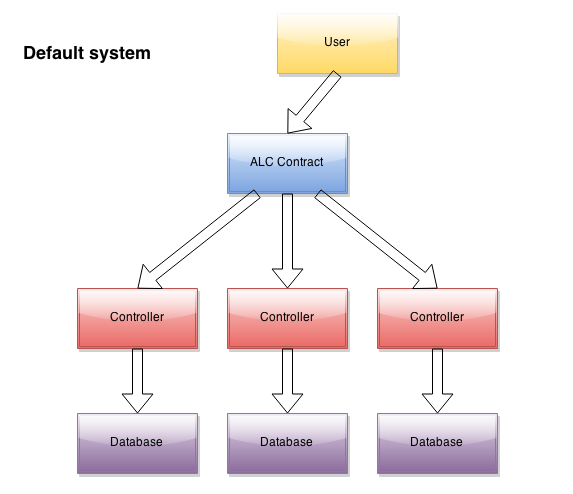
\includegraphics[width=\textwidth]{Figures/FiveTypesSystem}
\decoRule
\caption[]{}
\label{fig:FiveTypesSystem}
\end{figure}

\begin{figure}
\centering
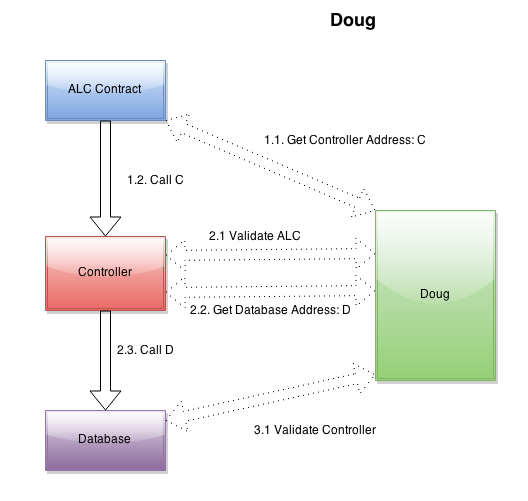
\includegraphics[width=\textwidth]{Figures/FiveTypesDOUG}
\decoRule
\caption[]{}
\label{fig:FiveTypesDOUG}
\end{figure}

Figure \ref{fig:FiveTypesSystem} (taken from Eris industries tutorials - see ref) shows a dependency graph between different components of a generic smart contract system built following the five types contract design pattern. Figure \ref{fig:FiveTypesDOUG} (also taken from Eris industries tutorials) shows how various components within a five type model interact with one another including with the contract management contract (here called Doug). Contracts confer with Doug to both validate the address of the calling contract and also to retrieve the address of any other contracts they themselves need to call.

\subsubsection{Benefits}
The principle benefit of the Five Types design pattern is modularity. Before calling code from another system component every contract first confers with the CMC to retrieve the correct address. This means that so long as the existing API is still supported, a system administrator can update the CMC with new component addresses and the whole system will continue to work.\\

An additional benefit of the Five Types design pattern is permissioned access. The CMC makes it easy for contracts to check the identity of a calling contract and terminate execution if it is foreign or unauthorised. \\


\subsubsection{Critiques}
Modularity comes at a cost. By introducing extra calls and more processing, the Five Types pattern increases the cost of execution. Modularity also introduces a degree of trust. A modular system must give some agent(s) the power to to update the behaviour of smart contract system. Of course, from a technical standpoint any changes made to the system will be publicly visible but practically, if the system is changed in a malicious way without formal notification, many users could suffer. There is a trade off between the flexibility of smart contract systems and the degree of trust-less ness provided to the user. This is an important practical consideration for pretty much all Ethereum based applications! \\

The Five Types also suffers from some scalability issues. Consider the example system illustrated in Figure \ref{fig:FiveTypesSystem}. If each controller had four functions in it's API and we had 10 controllers, the ALC would need 40 function calls in order to access them all. Furthermore, the addition of a new controller or the modification of an existing one would require the entire ALC to be swapped out. \\

The five type model is one example of a smart contract design pattern that is useful for exemplifying important concerns when building smart contract systems. More design patterns such as 'action driven architecture'\cite{ActionDriven}, have already been suggested to address some of the issues surrounding scalability. As the craft of dapp development matures, we will hopefully see many more useful patterns emerge. 




% Chapter 

\chapter{Go-op} % Main chapter title
\label{Goop} % For referencing the chapter elsewhere, use \ref{Chapter1} 

This chapter introduces the Go-op application in it's current state of development.

%%%%%%%%%%%%%%%%%%%%%%%%%%%%%%%%%%%%%%%%%%%%%%%%%%%%
\section{Welcome Page}
\begin{figure}
\centering
\makebox[\textwidth][c]{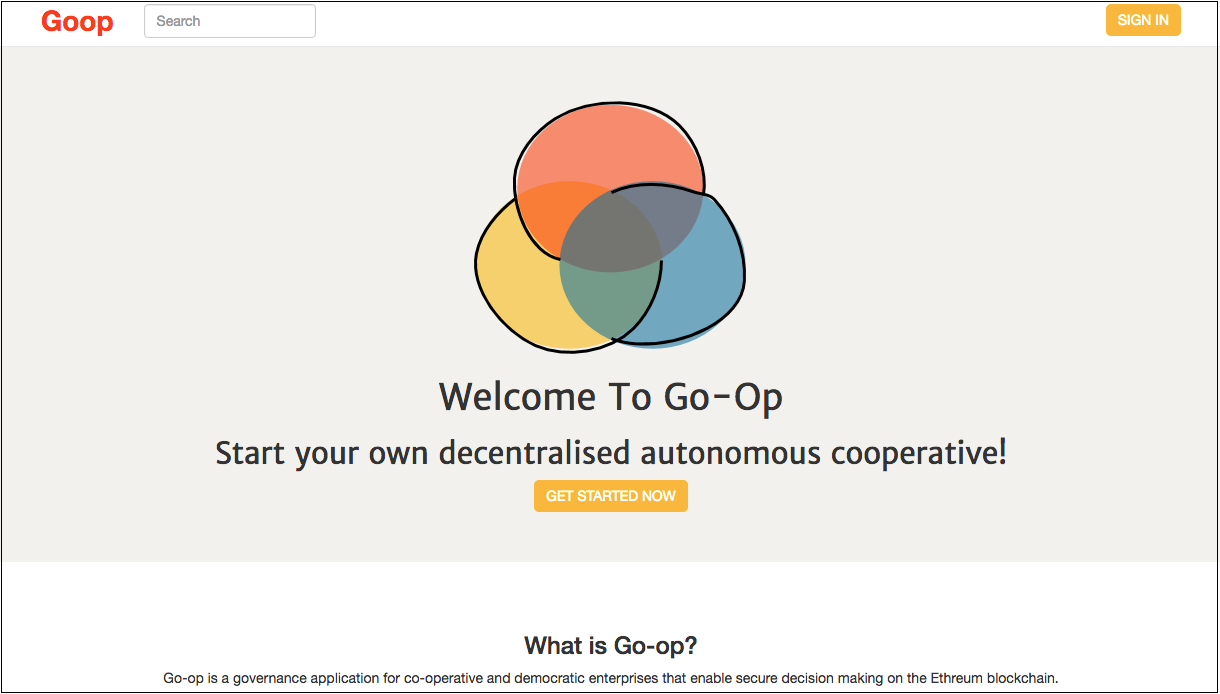
\includegraphics[width=1.4\textwidth]{Figures/WelcomePage}}
\decoRule
\caption[]{}
\label{fig:welpage}
\end{figure}

The landing or welcome page for Go-op is shown in Figure \ref{fig:welpage}. This is the first page a user will see when they load the application. It's purpose is to attract the users attention and describe the premise of the Go-op. By clicking the orange buttons to 'sign up' or 'get started now', the user will be taken to the registration page.\\

%%%%%%%%%%%%%%%%%%%%%%%%%%%%%%%%%%%%%%%%%%%%%%%%%%%%
\section{Registration}
\begin{figure}
\centering
\makebox[\textwidth][c]{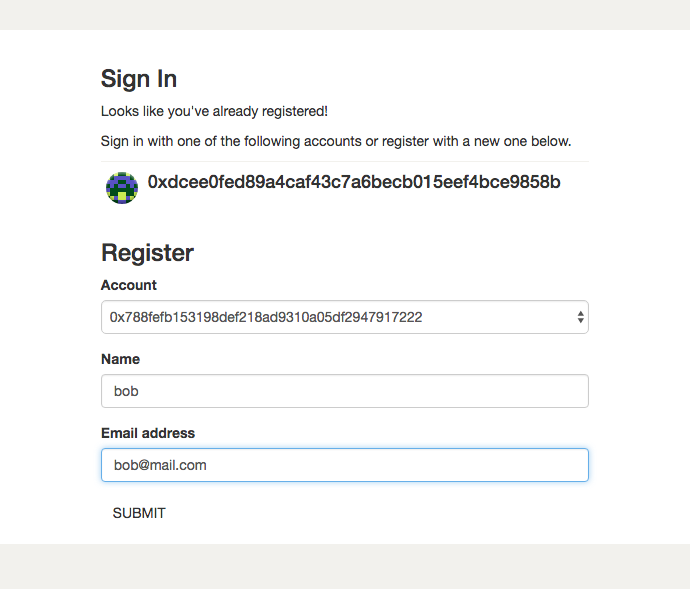
\includegraphics[width=1.4\textwidth]{Figures/RegistrationPage2}}
\decoRule
\caption[]{}
\label{fig:regpage}
\end{figure}

Users 'sign up' to Go-op through the registration page, figure \ref{fig:regpage}. The registration process associates a user's Ethereum account with their personal details. Ethereum accounts are managed by an external entity such as the local Ethereum client or by a Web3 browser such as Mist. Users are able to register an identity for each of their Ethereum accounts.\\

The only personal details currently required by Go-op are name and email address. Our research into membership application forms found that the information gathered by most coops is usually a name, address, telephone number and email. At this stage in development it is not yet clear whether a subset of this information will be sufficient for digital governance. It was decided that the PoC should be kept as simple as possible without introducing too many unvalidated features. 

% Future development work should proceed in tighter communication with cooperatives to vali

%%%%%%%%%%%%%%%%%%%%%%%%%%%%%%%%%%%%%%%%%%%%%%%%%%%%
\section{Home Page}

\begin{figure}
\centering
\makebox[\textwidth][c]{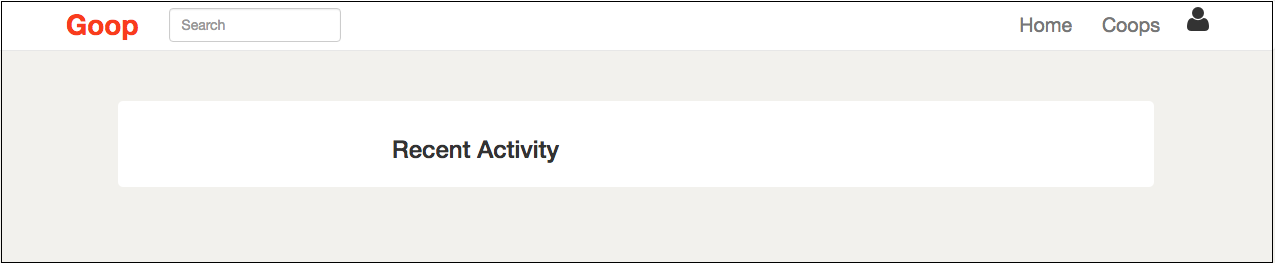
\includegraphics[width=1.4\textwidth]{Figures/HomePage}}
\decoRule
\caption[]{}
\label{fig:homepage}
\end{figure}

The user 'home page', shown in figure \ref{fig:homepage}, currently has no functionality. In future, the homepage should act as a quick reference panel for a user to identify recent changes with their co-operatives. The information we hope to populate this page with are new membership events, new proposal creation events and new proposal conclusion events.\\
 
%%%%%%%%%%%%%%%%%%%%%%%%%%%%%%%%%%%%%%%%%%%%%%%%%%%%
\section{My Coops}

\begin{figure}
\centering
\makebox[\textwidth][c]{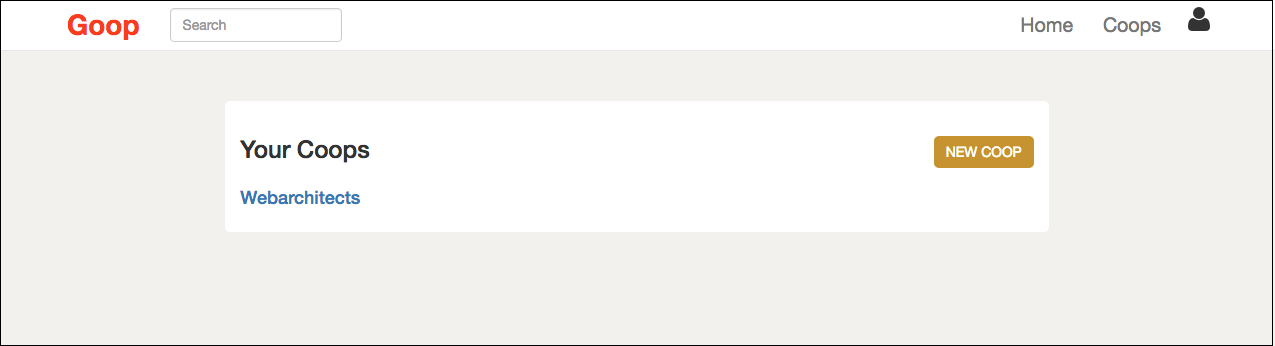
\includegraphics[width=1.4\textwidth]{Figures/MyCoopsPage}}
\decoRule
\caption[]{}
\label{fig:coopspage}
\end{figure}

The 'my coops' page, shown in figure \ref{fig:coopspage}, is a simple navigation page that displays all the co-operatives a user is a member of. Figure \ref{fig:coopspage} shows that the logged in user is a member of one co-operative called 'Webarchitects'. Users can set up a new co-operative on this page by clicking the 'new coop' button.\\

\subsection{Creating A Coop}

\begin{figure}
\centering
\makebox[\textwidth][c]{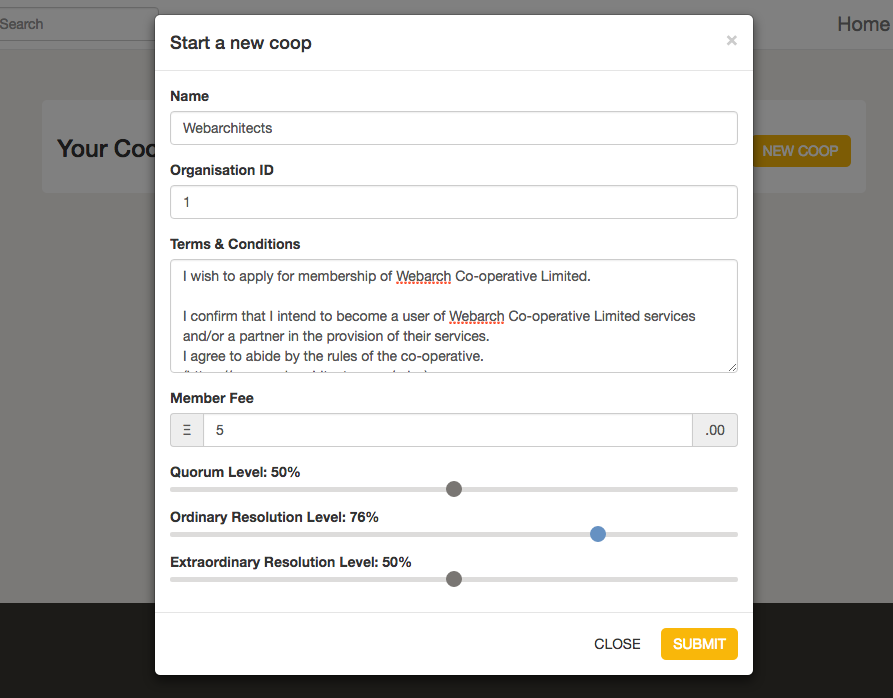
\includegraphics[width=1.4\textwidth]{Figures/CreateCoopPage}}
\decoRule
\caption[]{}
\label{fig:createcooppage}
\end{figure}

Figure \ref{fig:createcooppage} shows the pop up modal for creating a new co-operative. To set up a new co-operative a user must provide a name, Coops UK ID, Terms \& Conditions (for membership), membership fee (in Ether), quorum level and resolution levels (see section \ref{subsec:CooperativeGovernance} for more information).\\

The terms and conditions and membership fee are made visible to users when they join a co-operative. The quorum and normal resolution levels are used by Go-op to determine whether ordinary proposals tabled by members of the co-operative are passed or defeated. The extraordinary resolution level is not currently used by Go-op. In future, Go-op could allow it's members to table a second type of proposal to change the 'rules' of the co-operative itself (such as changing the quorum level). The extraordinary resolution level would define the level of agreement required for these kinds of proposals to pass. \\

The Coops UK ID is also not currently used by Go-op. At the moment, anyone can set up a co-operative on Go-op but in future, assurances around 'co-operative identity' may become a requirement. Because all real co-operatives should already have a Coops UK ID, providing it during creation could allow Coops UK to easily validate co-operatives signing up to Go-op.\\
 

%%%%%%%%%%%%%%%%%%%%%%%%%%%%%%%%%%%%%%%%%%%%%%%%%%%%
\section{Coop Page}

\begin{figure}
\centering
\makebox[\textwidth][c]{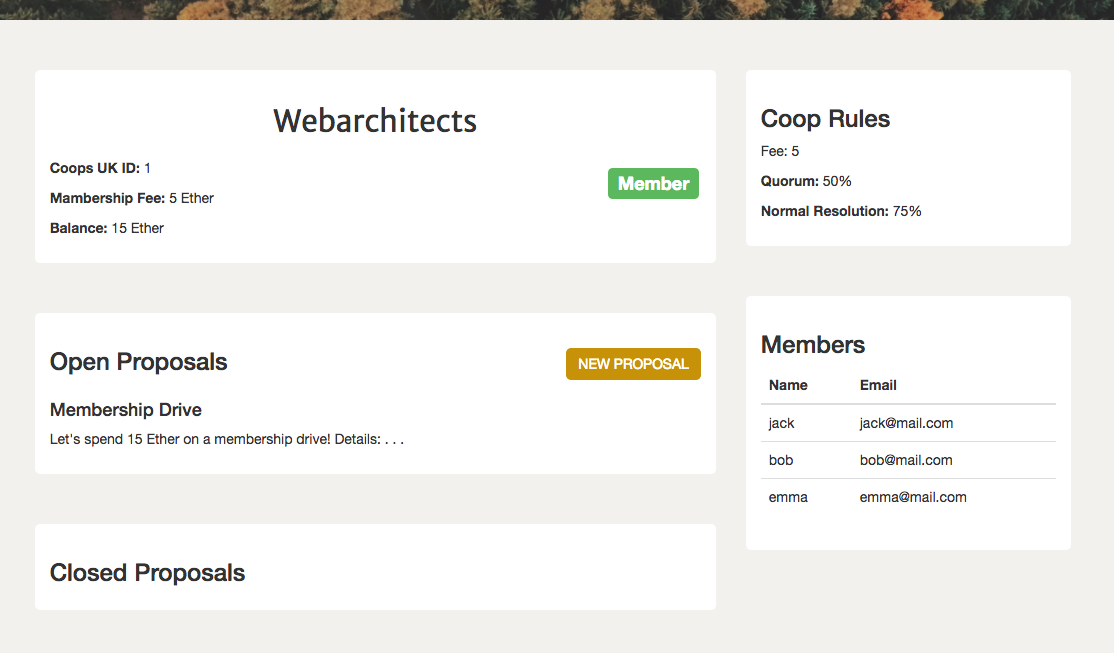
\includegraphics[width=1.4\textwidth]{Figures/CoopPage2}}
\decoRule
\caption[]{}
\label{fig:cooppage}
\end{figure}

Figure \ref{fig:cooppage} shows the home page for a co-operative. The page is split into five sections: title, rules, members, open proposals and closed proposals. The title section displays key information such as the name of the cooperative, it's balance (accumulated membership fees etc), it's membership fee and it's Coops UK ID. The 'rules' section lists the rules for quorum and resolution. The 'members' section is simply a list of members. The open proposals allows users to view proposals for which voting is still open and allows users to table new proposals. The closed proposals serves as an audit for closed and decided proposals. \\

\subsection{Creating A Proposal}

\begin{figure}
\centering
\makebox[\textwidth][c]{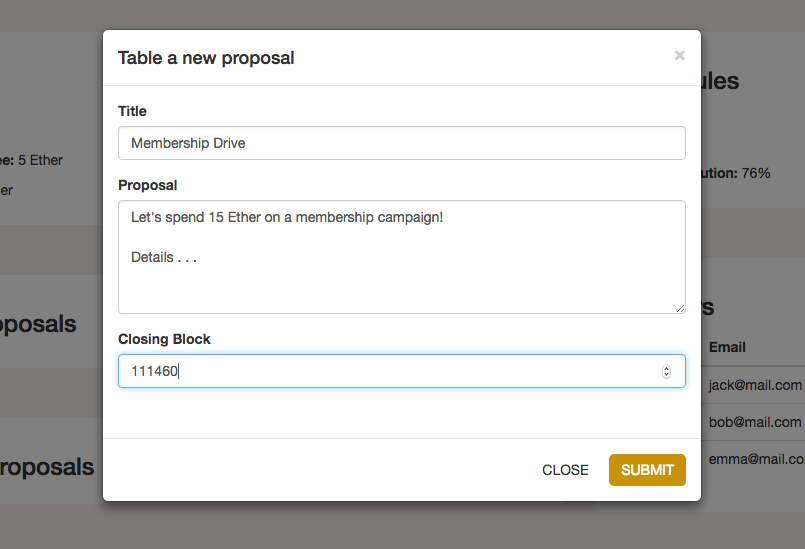
\includegraphics[width=1.4\textwidth]{Figures/NewProposalPage}}
\decoRule
\caption[]{}
\label{fig:createproposal}
\end{figure}

Clicking on the 'new proposal' button in the 'open proposals' section opens the 'new proposal' dialog shown in figure \ref{fig:createproposal}. This is a simple form with three fields: title, proposal text and closing block. The closing block determines the block on which the vote is scheduled to close. Because Go-op uses the Ethereum Alarm Clock as the underlying scheduling system (see section\ref{sec:blocktime}), a block number is the most precise way a closing date can be specified. This is reasonably ugly feature that pierces the abstraction of blockchain technology from end users. Ideally, users should specify closing dates in terms of time. This may be possible if Go-op switches to a lazy evaluation approach as discussed in section \ref{sec:blocktime}. At the very least, the form should provide extra information about the estimated processing dates for any block in the future. 
 

\subsection{Voting On A Proposal}
\begin{figure}
\centering
\makebox[\textwidth][c]{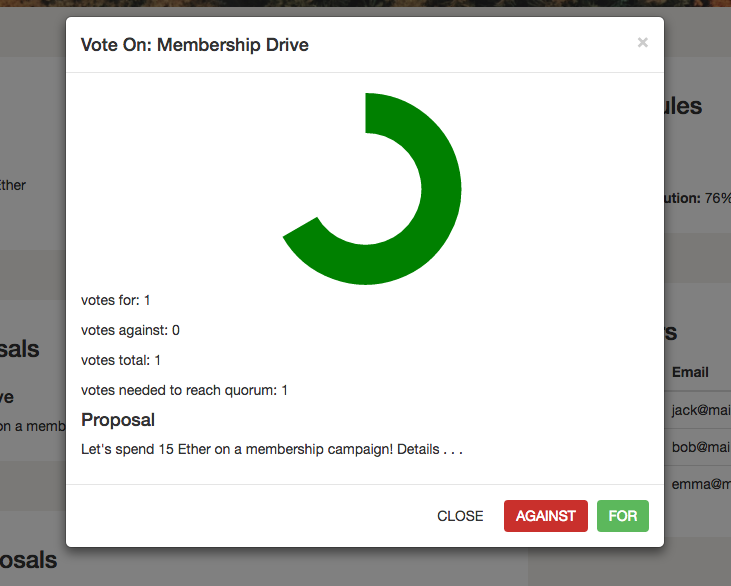
\includegraphics[width=1.4\textwidth]{Figures/ProposalVotePage}}
\decoRule
\caption[]{}
\label{fig:proposalvote}
\end{figure}

Figure \ref{fig:proposalvote} shows the pop up for an open proposal. The pop up includes information on the actual proposal as well as the number of votes for, votes against, total votes and number of votes required to reach quorum. This information is also summarised graphically in a simple 'doughnut' chart. The empty space in the doughnut chart illustrates the percentage of votes still required to reach quorum. There are three buttons at the foot of the pop up which allow a user either close the pop up or vote for or against the proposal.\\

When a proposal closes it becomes listed in the 'closed proposals' section of the coop home page. Pop ups for closed proposals look identical as for open proposals except that there are no buttons for voting.\\

\section{Loading Screens}
\begin{figure}
\centering
\makebox[\textwidth][c]{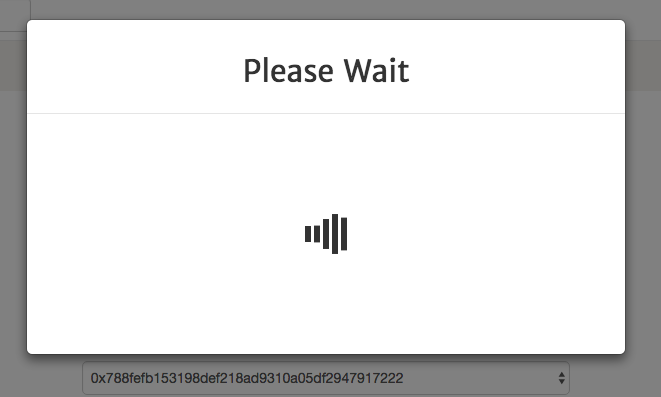
\includegraphics[width=1.4\textwidth]{Figures/WaitPage}}
\decoRule
\caption[]{}
\label{fig:waitpage}
\end{figure}

Many user interactions spawn transactions that need to be mined into the blockchain. Loading modals, such as the one shown in figure \ref{fig:waitpage}, are used to avoid unresponsive views while the application waits for transactions to be processed. Whilst this is nice, transactions can take up to thirty seconds to get mined which is a long time to look at a loading screen. A better solution for the future would be an optimistic UI that simply assumes transactions will be successful when it can be confident. Some kind of icon could be used to show which aspects of the UI have been confirmed in the blockchain and which components are still pending.
















 
% Chapter 5 implementation

\chapter{Implementation} % Main chapter title

\label{Implementation} % For referencing the chapter elsewhere, use \ref{Chapter1} 

\section{Architecture}
\begin{figure}
\centering
\makebox[\textwidth][c]{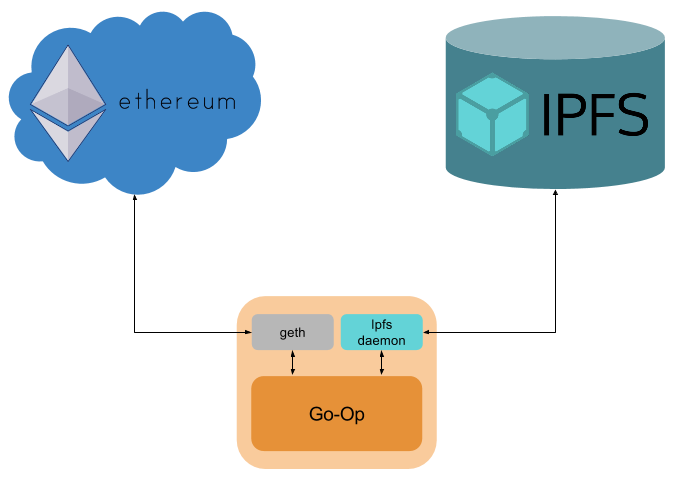
\includegraphics[width=1.2\textwidth]{Figures/GoopArch}}
\decoRule
\caption[Go-op Architecture Diagram]{Go-op architecture diagram - 'geth' Ethereum client, IPFS node and Go-op 'front end' all run on local host machine.}
\label{fig:GoopArch}
\end{figure}

Figure \ref{fig:GoopArch} is a high level illustration of the Go-Op application architecture. It is a simple distributed architecture and notable for the lack of any client server asymmetry. The Ethereum cloud represents the Ethereum peer to peer network and the large IPFS database represent the IPFS network similarly. The 'host machine' must run both an Ethereum and IPFS client in order to participate in the respective networks. The Go-op application is a typical javascript/HTML/CSS web application and can therefore be run in a normal Internet browser. \\

Go-op is very much a proof of concept application and currently requires the manual installation of both an Ethereum and IPFS client. Users are not generally expected to engage in such low level technical processes but it is practical limitation for the time being. The idealised Web3 architecture (discussed in section \ref{sec:web3Arch}) outlines a better vision for user interaction with new tools such as the Mist browser which is planned to be released later this year. In figure \ref{fig:GoopArch} Mist would be represented by the light orange box surrounding the host processes. The Mist browser will internally manage the Web3 clients to hide unnecessary complexity from the application users. \\

The Go-op 'front end' code interacts with the local Ethereum node through the web3.js library\cite{Web3JS}. The web3.js library implements the Web3 Javascript API\cite{JavascriptAPI} which is well documented online (see ref). Under the hood, the web.js library communicates with the local Ethereum instance via RPC (remote procedure calls). Communication between Go-op and the IPFS client is achieved through the ipfs-js\cite{ipfs-js} library, developed by ConsenSys (a leading blockchain technology company developing on Ethereum). The ipfs-js library is a simple wrapper around official ipfs client javascript library but adds some nice Ethereum specific utilities such as conversions between hex (format for Ethereum storage) and base58 format of Ipfs addresses. \\

One important note is that user accounts are not managed through the web3 library and must be added / removed etc through the Ethereum client command line interface. User accounts need to be unlocked before they can be used by the Go-op application to sign transactions. Again, the development of new user friendly interfaces will soon make it possible to avoid such pains. \\

For more information about installing and running Ethereum and IPFS clients consult Appendix A. \\

A possible alternative to running Web3 clients locally is to run them as web services (this is the kind of approach offered by Block apps\cite{BlockApps} for example). Whilst this has the potential to simplify the problem in the short term, it generally works against the objectives of decentralisation. The process introduces the web service as a 'trusted' intermediary. It is counter intuitive to add points of trust into the process of executing Ethereum contracts as the whole point is to eliminate 'centralised trust' in the first place. \\

Lower level architecture explanations for the Go-op application and smart contract system are provided in the following sections. \\

\section{Go-op Smart Contract System}
The smart contract system for Go-op (Figure \ref{fig:SCArch}) is relatively small. It is composed of five static contract accounts (CMC, UserController, UserRegistry, CoopRegistry and MembershipRegistry) and a dynamic number of user and CoopContract accounts. The architecture of the contracts roughly follows the Five Types design pattern discussed in section \ref{sec:scDesign}.\\ 

The principal entities in the system are users and 'coops' which are stored in the UserRegistry contract and CoopRegistry contract respectively. The many to many 'membership' relation between users and coops is stored by the MembershipRegistry contract. The next few subsections explain the role of each system component in detail.\\

\begin{figure}
\centering
\makebox[\textwidth][c]{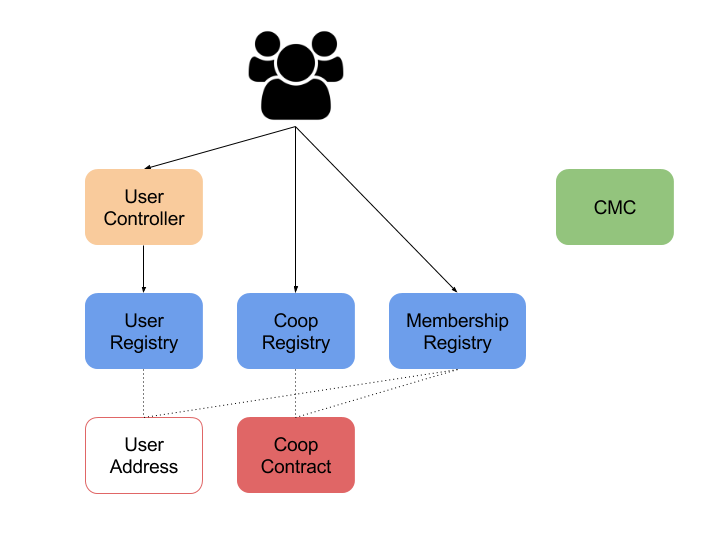
\includegraphics[width=1.2\textwidth]{Figures/SCArch}}
\decoRule
\caption[Go-op Smart Contract System Architecture]{Go-op smart contract system architecture.}
\label{fig:SCArch}
\end{figure}

\subsection{CMC}
Although it was not possible to fully realise the Five Type design pattern due to practical limitations (discussed shortly), Go-op still makes use of a CMC (contract management contract) to help manage modularity and permissions. Essentially, the CMC holds a mapping of component names to contract addresses. Only the owner of the CMC, that is the account that created it, is able to add, remove and 'dissolve' contracts. The CMC contract is a standard component of the Five Types pattern. For a code listing and detailed explanation see the Eris Industries tutorial \cite{FiveTypes}.

\subsection{CMCEnabled}
CMCEnabled is an 'abstract' contract that is inherited by all non CMC contracts. It defines a minimal interface required by the CMC to interact with non CMC contracts. A ContractProvider contract is used to define the minimal interface required in the opposite direction. Again, these are also standard contracts of the Five Types pattern. A code listing and detailed explanation be found here\cite{FiveTypes}.\\

\subsection{UserRegistry \& UserController}
The UserRegistry contract (Figure \ref{fig:UserRegistry}) is very simple. It stores a mapping of user account addresses to IPFS addresses and has two functions, setUserData and getUserData (not shown in figure), for reading and writing to this mapping. The UserRegistry uses the CMC contract to restrict both read and write permission to only the UserController contract. \\

\begin{figure}
\centering
\makebox[\textwidth][c]{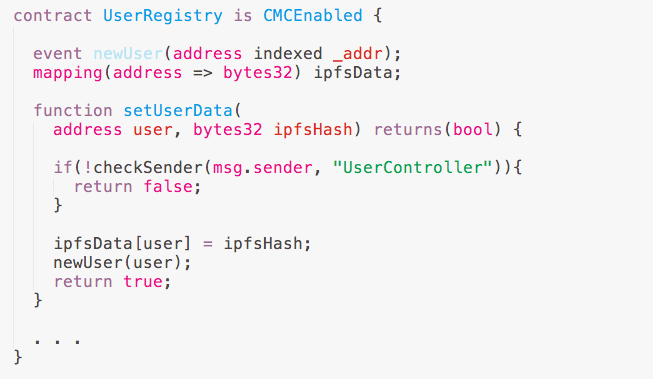
\includegraphics[width=1.4\textwidth]{Figures/UserRegistry}}
\decoRule
\caption[UserRegistry Contract Snippet]{Snippet of the UserRegistry contract}
\label{fig:UserRegistry}
\end{figure}

The UserController is, for now, simply a wrapper for the UserRegistry contract. It does not provide any additional logic and was included in an attempt to follow the Five Types pattern (section \ref{sec:scDesign}). Although it is a redundant component, the process of adding a user controller to the system revealed some practical limitations to composing smart contract systems. Critically, the possible return types between contracts executing in the EVM are different to the returnable types for external calls. To be specific, variable length arrays, which includes strings and byte arrays, are not possible return types between contracts executing within the EVM but are permitted return types for direct calls from externally owned accounts. \\

Because IPFS addresses are 34 bytes long and the largest fixed size byte array in Solidity is 32 bytes, it is not possible to pass a whole IPFS address between the UserRegistry and the UserController contracts. This is a big issue for dapps that use IPFS but also want to follow modular design patterns that require contract interaction. \\

There are a few possible 'workarounds' in this case:\\

\begin{enumerate}[label=(\alph*)]
\item Remove the UserController completely and read straight from the registry. From a design perspective this is a somewhat degenerate solution. \\

\item Add logic to the UserController that splits and re-combines the IPFS hash on saving and retrieving from the UserRegistry. This would require the UserRegistry to implement two methods for returning different parts of the IPFS hash e.g \code{first32\allowbreak IPFSbits()}, \code{next2\allowbreak IPFSbits()}. This is not an ideal solution because adding processing to deconstruct and reform byte arrays in the UserController would increase the gas requirements and therefore the costs of the system. \\

\item Only store the last 32 bytes in the blockchain. This is possible because IPFS hashes are 'self-describing' and the first 2 bytes just defines the hash function used. For all current intents and purposes this is always SHA-256. The hex string that represents SHA-256 within IPFS, '0x1220', is simply dropped and re-appended on writing and reading from Ethereum. This is an easy to implement solution and is the workaround currently employed by Go-op for the UserController and UserRegistry. However, it only works in this specific case for IPFS addresses and doesn't solve the dynamic array return type problem in general.\\
\end{enumerate}

There are plans to implement dynamic return types between contracts in a future protocol update so, hopefully, the current workaround is only temporary\cite{ReturnArray}. A big factor for choosing workaround c) is that it will be the easy to revert once the protocol is updated.\\

\subsection{CoopRegistry}
The CoopRegistry is another relatively simple contract. It stores the addresses of all CoopContract contracts in the Go-op system. Unlike the UserRegistry it does not store any additional information about cooperatives, such as an IPFS address, because this is stored by the individual CoopContracts themselves. The CoopRegistry contract exposes two methods: \code{newCoop()} and \code{getCoops()}. \\

\code{getCoops()} returns the state variable array of CoopContract addresses. \\
 \begin{figure}
\centering
\makebox[\textwidth][c]{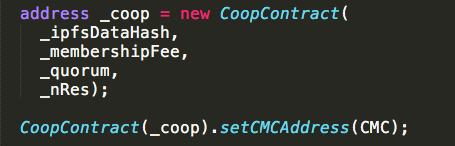
\includegraphics[width=1.4\textwidth]{Figures/CoopRegistry}}
\decoRule
\caption[CoopRegistry Coop Creation Snippet]{Snippet of the CoopContract creation within the CoopRegistry contract (a Solidity definition for CoopContract must be provided in order to compile CoopRegistry) }
\label{fig:CoopRegistry}
\end{figure}

\code{newCoop()} creates a new instance of a CoopContract with the provided parameters (see Figure \ref{fig:CoopRegistry}) and saves the resultant address in the registry array.\\

A cleaner 'separation of concerns' might be achieved here by extracting the complexity of CoopContract creation out of the CoopRegistry into a CoopController. This could help modularity by creating a more rigid API for the CoopRegistry and would abstract the registry contract from the public facing API. However, assuming the avoidance of intensive contract code[Footnote] it is not possible to pass variable length arrays, such as the list of coop addresses, between contracts. This means that at least some part of the public facing API must be exposed by the CoopRegistry directly. At present therefore, a new coop controller contract probably does not simplify the design of the system enough to warrant its introduction. \\

The CoopRegistry does not currently implement a \code{removeCoop()} function. Whilst this may be desirable in future, at present, the precise conditions for removing a coop from the Go-op system are not well understood. \\

\subsection{MembershipRegistry}
The MembershipRegistry contract maintains the many to many 'membership' relationship between users and cooperatives. It is slightly more involved than the other registry contracts as it stores more information, handles more advanced queries and needs to manage payment of membership fees. Figure \ref{fig:MemRegVars} illustrates the state variables of the MembershipRegistry. The relationship is stored in both directions to reduce computation when retrieving membership information. \\

\begin{figure}
\centering
\makebox[\textwidth][c]{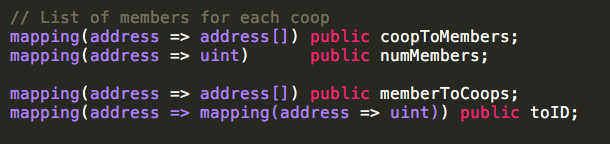
\includegraphics[width=1.4\textwidth]{Figures/MemRegVars}}
\decoRule
\caption[MembershipRegistry State Variables]{State variables of the MembershipRegistry smart contract.}
\label{fig:MemRegVars}
\end{figure}

The MembershipRegistry has five methods \code{register()}, \code{deregister()}, \code{getMembers()}, \code{getCoops()}, \code{idOf()}, \code{totalMembers()} and \code{isMember()}. \\

\code{register()} stores a new relationship between a user and a coop. Registration is successful after a number of checks are completed:
\begin{enumerate}
\item Check with the UserRegistry and CoopRegistry that the calling account is a registered user and that the address of the coop being joined is a CoopContract within the Go-op system.

\item Read the membership fee from the CoopContract of the cooperative being joined. If the value sent with the transaction is not exactly equivalent to the fee then an exception is thrown which causes the inexact fee to be returned to the sender. 

\item Check the member is not joining twice by iterating through all the coops already associated with a member.

\item Forward the membership fee to the CoopContract being joined.

\item Finally, the registry data is updated to reflect the new membership.
\end{enumerate}

The \code{deregister()} method removes the sender as a member of the given coop. In future it is likely that more complex de-registration functionality will be required such as membership termination by group consensus.\\

\code{getMembers()} and \code{getCoops()} are explicit methods for accessing the registry data structs. Again, the need to return variable length arrays removes the practical possibility of a MembershipController contract at this time. \\

The \code{isMember()} method is required by CoopContracts to establish membership during voting.\\

\subsection{CoopContract}
Each cooperative in the Go-op system exists as a unique CoopContract (full listing in section X). The CoopContract is by far the most complex contract because it implements a proposal voting system. The  contract has twelve methods: \code{set\allowbreak CoopData()}, \code{get\allowbreak CoopData()}, \code{get\allowbreak ProposalData()}, \code{get\allowbreak VotesFor()}, \code{getVotes\allowbreak Against()}, \code{has\allowbreak Passed()}, \code{has\allowbreak Failed()}, \code{isA\allowbreak Member()}, \code{getNum\allowbreak Members()}, \code{new\allowbreak Proposal()}, \code{support\allowbreak Proposal()}, \code{close\allowbreak Proposal()}. The majority of these methods are one liners and fairly self explanatory. The most involved functions are \code{new\allowbreak Proposal()}, \code{support\allowbreak Proposal()}, \code{close\allowbreak Proposal()} which will be discussed presently.\\
\begin{figure}
\centering
\makebox[\textwidth][c]{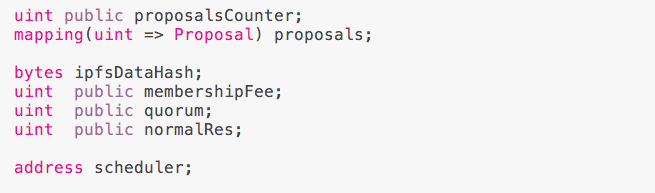
\includegraphics[width=1.4\textwidth]{Figures/CoopState}}
\decoRule
\caption[State Variables ofCoopContract]{State variables of the CoopContract.}
\label{fig:CoopState}
\end{figure}

Figure \ref{fig:CoopState} shows the state variables of a CoopContract. The ipfsDataHash holds an IPFS address for non logic-critical information (such as terms and conditions). The membership fee is stored in Wei (a sub denomination of Ether) and the quorum, normal resolution and extraordinary resolution levels are all stored as percentages (integers between 0 and 100). Proposals are stored in the proposals mapping. Figure \ref{fig:ProposalStructs} shows the Proposal and ProposalVotes structs. The textual information for a proposal is also stored in IPFS and it's address is stored in the Proposal struct.\\

\begin{figure}
\centering
\makebox[\textwidth][c]{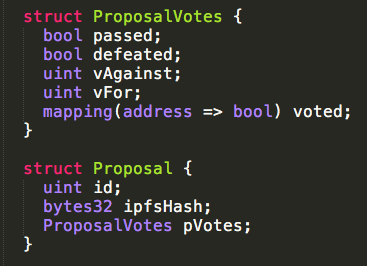
\includegraphics[width=1.4\textwidth]{Figures/ProposalStructs}}
\decoRule
\caption[Proposal Structs in CoopContract]{Proposal structs used by the CoopContract.}
\label{fig:ProposalStructs}
\end{figure}

Proposals are created through the \code{newProposal()} method. The process of this method can be broken down into three stages: 
\begin{enumerate}
\item First, it checks the caller is a member of the cooperative via a call to the \code{isMember()} function of the \keyword{MembershipRegistry}. If the caller is not a member then the function call returns immediately. 
\item Secondly, it creates a new Proposal struct from the provided arguments and adds it to the proposals mapping with a new id taken from the proposalsCounter. 
\item Finally, and most interestingly, it schedules a call with the Ethereum alarm clock service to close the proposal at a future block. When the given block number is reached, the Ethereum Alarm Clock service will call the \code{closeProposal()} method on the \keyword{CoopContract}. The Ethereum Alarm Clock service and the challenge of measuring time on a blockchain is discussed at greater depth in section \ref{sec:blocktime}
\end{enumerate}

Votes for proposals are registered with the \code{supportProposal()} function. The behaviour of this function can also be broken down into three stages:
\begin{enumerate}
\item First, it follows the same process as \code{newProposal()} to check the caller is a member of the cooperative.
\item Secondly, it checks if the proposal has not already ended and that the sender has not already voted. If either are true, the function returns.
\item Finally, based on the call parameters, it registers the vote by incrementing either the vFor or vAgainst field of the proposal.\\
\end{enumerate}

The \code{closeProposal()} function is used to close a proposal and determine whether it has passed or been defeated. As described in the description for \code{newProposal()}, this function is triggered by the Ethereum Alarm Clock service. The function proceeds as follows:
\begin{enumerate}
\item The member count is retrieved from the \keyword{MembershipRegistry}. 
\item If the proportion of votes to member count does not surpass the quorum level (see ) then the proposal is closed as defeated. 
\item If quorum is reached and the proportion of 'votes for' to total votes surpasses the normal resolution level (see ) then the proposal is closed as passed, otherwise it is defeated.
\end{enumerate}

In future, the proposal system of the CoopContract could be extended to also allow coops to pass proposals that change the rules of the coop itself (such as the normal resolution level). A new extraordinary resolution level would be required to pass these kinds of special proposals.\\

\section{Client Application}
\subsection{Meteor Framework}
As discussed in 'idealised Web3.0 architecture' (Section \ref{sec:web3Arch}), the 'front end' of an Ethereum dapp is typically built with the same technology stack as that of a traditional web application and therefore is very much compatible with existing browsers. Despite this, a number of popular dapp specific framework choices have emerged from the community (such as Embark\cite{Embark}, Truffle\cite{Truffle} and Meteor\cite{Meteor}) which supposedly offer added usability for Ethereum development (such as integration of test harnesses for Solidity smart contracts). A certain amount of time was necessarily dedicated to the exploration of these frameworks during the initial stages of Go-op development. More information about this investigation can be found in Appendix A.\\

The framework chosen for the development of Go-op was Meteor\cite{Meteor}. Meteor is a 'full stack' javascript application platform that includes a 'key set' of technologies and libraries and a dedicated build tool. The distinguishing feature of the Meteor platform is its emphasis on SPAs (Single Page Applications) and data on the wire, which helps developers easily manage data collections across the client and server. The motivation for using Meteor was based on its popularity within the community (used by established projects including Boardroom see \ref{subsec:boardroom}), the number of supporting libraries and boilerplates and recommendations from Ethereum developers\cite{MeteorRef}.\\

Meteor has recently updated from version 1.2 to 1.3. The update changed the behaviour of the build tool and introduced support for ES2015 modules and npm packages out of the box. Go-op has been developed with Meteor 1.3 in order to future proof as much as possible and embrace the improved compatibility with ECMAScript 6.\\

\subsection{Application Structure}
\begin{figure}
\centering
\makebox[\textwidth][c]{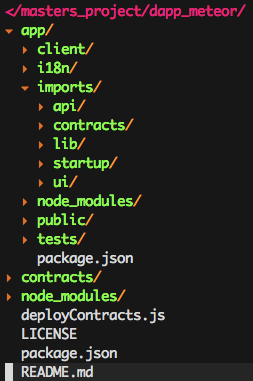
\includegraphics[width=0.5\textwidth]{Figures/AppStructure}}
\decoRule
\caption[Front End Application Structure]{Front end application structure}
\label{fig:AppStructure}
\end{figure}

Figure \ref{fig:AppStructure} shows the main folders in the Go-op project. This is a typical Meteor 1.3 organisation and should be easily navigable to any developer familiar with the Meteor stack. The role of the various project folders within the app folder are as follows: \\

\begin{itemize}
\item \keyword{client} - name sensitive folder used by the meteor build system.
\item \keyword{I18n} - used by meteor package to enable easy internationalisation of application.
\item \keyword{Imports} - main folder that contains bulk of client side logic. 
\begin{itemize}
\item \keyword{api} - contains database modules and event reactors that form an abstraction layer between the template or view logic and the Ethereum and IPFS interaction code.
\item \keyword{contracts} - This is the destination folder for the compiled 'contract modules' that are generated as part of the deployment script see \ref{subsec:deployScript}.
\item \keyword{lib} - some internal and external library code.
\item \keyword{startup} - common meteor folder. Holds key application files including startup logic and front end routes.
\item \keyword{ui} - contains the template files for the application views.  
\end{itemize}
\item \keyword{contracts} - Contains solidity smart contracts.
\item \keyword{deployContracts.js} - script for compiling, building and deployment of smart contracts see \ref{subsec:deployScript}.
\end{itemize}

Node\_modules, readme and package.json are standard javascript application assets. More information about the Meteor build system and conventions can be found in the guides, tutorials and documentation available at the meteor website.\\

\subsection{API}
This section describes the contents of the api folder which forms a layer between the application view logic and the Web3 'backend'.

\subsubsection{database}
The client side 'database' (as shown in figure X) abstracts complexity away from view logic by orchestrating the retrieval of data from the Web3 'backend' and exposing an easy to use, reactive and 'promisified' interface.\\

\begin{figure}
\centering
\makebox[\textwidth][c]{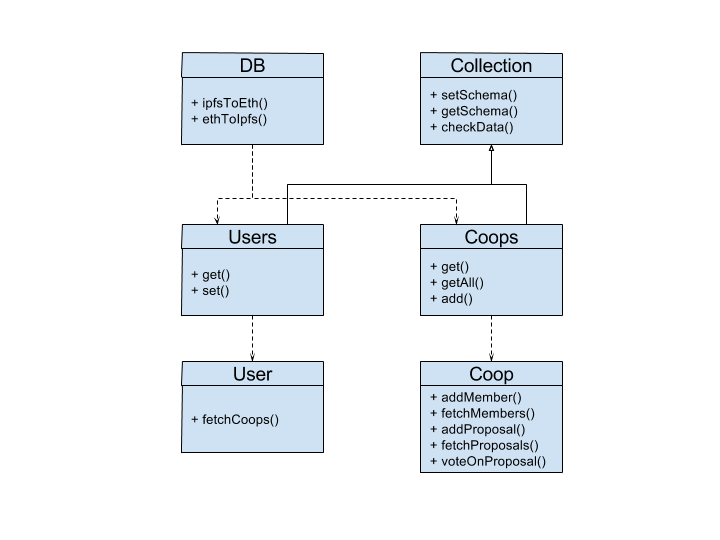
\includegraphics[width=1.4\textwidth]{Figures/dbClassDiagram}}
\decoRule
\caption[Front End Database Alass Diagram]{Front end database class diagram.}
\label{fig:dbClassDiagram}
\end{figure}

Figure \ref{fig:dbClassDiagram} shows the components of the database and the relationship between them. Listing \ref{lst:label} illustrates the API exposed to the view logic. Under the hood, the query first fetches the information for the coop at 'coopAddress' from the smart contract system and then uses it to consruct an in memory \code{Coop} object which it returns. \code{fetchMembers()} triggers another call to the smart contract backend to fill in all the information for a cooperatives members. The \code{Coop} object saves this information internally and then returns a reference to itself. \\

\begin{lstlisting}[caption={Example query to the front end database api}, label={lst:label}]
db.coops.get(coopAddress).then(function(coop) {
	return coop.fetchMembers();
}).then(function(coop) {
	// do something.
});
\end{lstlisting}

The \code{db} class is the entry point of the API. It creates an IPFS connection which it uses to construct the two database collections: \code{Users} and \code{Coops}. The \code{db} class constructs each of the Ethereum 'reactor classes' (discussed in the next section) which are also injected into the two collections. The \code{db} class has two helper functions for converting IPFS addresses between IPFS and Ethereum compatible formats.\\

\code{Collection} is an 'abstract' class that defines some common functionality for a collection, such as setting and checking schemas. Although there is no relational database per se, Go-op still uses schemas to avoid storing malformed data in the Web3 backend. Using schemas to validate on write avoids the need for excessive guard code upon reading, which is typically a more frequent operation.  Go-op uses the js-schema\cite{jsSchema} library for this purpose.\\

The design of the database api is partly inspired by Martin Fowler's Active Record pattern\cite{ActiveRecord} whereby tables and records from a relational database are reflected by in memory objects. The \code{Coops} and \code{Users} collections both implement a \code{get()} method which gathers the information from Ethereum and IPFS and then uses it to construct and return either a \code{Coop} or \code{User} object. \code{Coop} and \code{User} objects have an address field and correspond to real Ethereum accounts. They also have methods such as \code{fetchMembers()} or \code{fetchCoops()} which retrieve additional information from the 'backend' to 'fill in' the objects further.\\

Currently, the \code{Coops} and \code{Users} collections don't implement any level of caching. This means that every time the \code{get()} function is called the data is re-fetched from the Web3 backend. Caching database collections would improve the performance and user experience of Go-op but introduces additional challenges surrounding data consistency and cache invalidation.\\

Figure X illustrates the basic process of collecting data from Ethereum and IPFS. IPFS addresses are retrieved from Ethereum using the web3.js library and the compiled contract modules created by the deployContracts script (see section \ref{subsec:deployScript}). The IPFS address is then converted back into an IPFS friendly format and finally, the data is retrieved from IPFS (via the ipfs-js library) and used to construct in memory objects.\\

\subsubsection{Ethereum Reactors}
In order to explain the role of the \code{EthereumReactor} classes it is necessary to go into a brief aside about reactivity in Meteor. In this context, reactivity describes the ability of the application UI to automatically react or respond to changes in the underlying application data.\\

The native Meteor system follows a transparent reactive programming pattern. The reactive programming pattern can be understood as the interplay between reactive data sources, such as database queries, and reactive data consumers or reactive computation contexts. Reactive data sources record the computation context they are being accessed within. When the value of a reactive data source changes, such as the result of a database query, it triggers all its dependencies which causes all the computation contexts that access the reactive data source to re-run. For a more detailed explanation of transparent reactive programming in Meteor see \cite{Tracker}.\\

To help build reactive user interfaces in Go-op, the database is implemented as a reactive data source. This means that database queries in view templates (listing \ref{lst:label} for example) get re-run whenever the result of the query changes. The result of a query changes whenever data in the backend Ethereum contracts change. The role of the 'reactor classes' is to store dependencies created by database queries and trigger them when changes in Go-op smart contracts are detected. Changes to smart contracts are detected following the event pattern described in section \ref{subsec:events}. \\

\begin{figure}
\centering
\makebox[\textwidth][c]{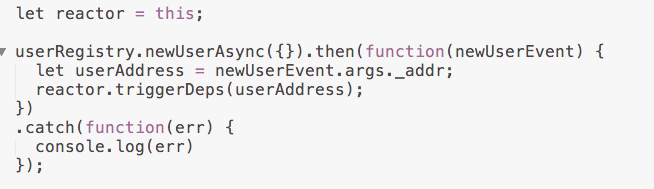
\includegraphics[width=1.4\textwidth]{Figures/UserRegistryReactor}}
\decoRule
\caption[Critical Section In UserRegistryReactor]{Critical section of UserRegistryReactor}
\label{fig:UserRegistryReactor}
\end{figure}

When a new user is added to a the \code{UserRegistry} the \code{newUser} event is fired (see Figure \ref{fig:UserRegistry}). Figure \ref{fig:UserRegistryReactor} shows the critical logic in the \code{User\allowbreak Registry\allowbreak Reactor} that listens for this event. When it fires, the \code{UserReactor} triggers all the reactivity dependencies that have been registered to it. \\

\begin{figure}
\centering
\makebox[\textwidth][c]{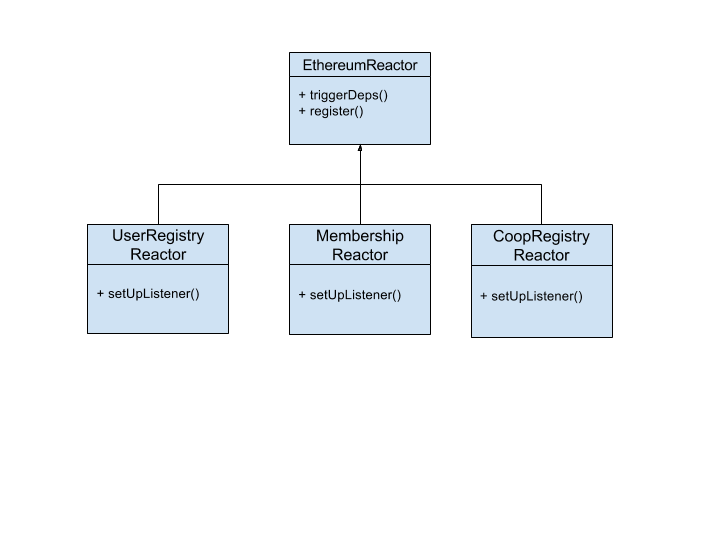
\includegraphics[width=1.4\textwidth]{Figures/ReactorsClassDiagram}}
\decoRule
\caption[Reactors Class Diagram]{Class diagram for Ethereum reactor classes.}
\label{fig:ReactorsClassDiagram}
\end{figure}

Figure \ref{fig:ReactorsClassDiagram} shows the class hierarchy for the various reactor classes. There are currently three reactor classes; one for each of the three registries in the smart contract system: \code{UserRegistryReactor}, \code{CoopRegistryReactor} and \code{MembershipReactor}. Each reactor extends the \code{EthereumReactor} class which defines common methods between all reactors for registering and triggering dependencies. \\

\begin{figure}
\centering
\makebox[\textwidth][c]{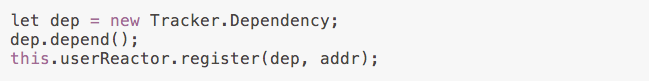
\includegraphics[width=1.4\textwidth]{Figures/UsersDepRegistration}}
\decoRule
\caption[Dependency Registration in Users Collection]{Snippet of Users collection highlighting reactive dependency registration process}
\label{fig:UsersDepRegistration}
\end{figure}

Figure \ref{fig:UsersDepRegistration} is a snippet from the \code{Users} database collection. It shows how the database becomes a reactive data source through creating a reactivity dependency and registering it with the \code{CoopRegistryReactor}. \\

An alternative approach to tracking reactivity dependencies manually would be to use an in browser database such as Minimongo (this is the approach taken by other dapps such as Boardroom). Minimongo collections are built specifically as reactive database sources for use in Meteor applications. Writing the data from the backend into Minimongo collections would remove the need to manually handle reactive dependencies at such a low level. The problem with Minimongo is that collection updates would not sync automatically with the Web3 backend. Write and delete operations would have to be duplicated; once for the Minimongo collection and once for the web3 backend. Although automatic reactivity would be convenient, trying to maintain two separate data stores consistently is an easy way to introduce bugs and has so far been avoided.\\

\subsection{User Interface}
The Go-op UI (User Interface) is divided into several views (see section). Each view is defined by a HTML template and a javascript controller. When Meteor builds the application is compiles the HTML templates into javascript objects. The view controllers use the Meteor Template library to access the compiled template objects. Template objects provide a number of different methods for executing functionality at different stages of a template lifecycle including a way to attache template helpers and event handlers. The actual rendering of templates is handled by the Blaze template engine. \\

Thanks to the database layer that has just been discussed, all of the logic in the view controllers is relatively simple. Data is retrieved from the 'database' and then used to render the template. Because the database is implemented as a reactive data source and, by default, template helpers as reactive data contexts, the view controller logic doesn't really have to worry about reactivity at all. When a reactive computation context needs to be created explicitly, such as within the template onCreated function, the Tracker library is used. \\

\subsection{User Experience}
User experience is extra important for blockchain based applications because of the significant delays introduced by transaction confirmation times. Users are accustomed to fast response times so creating an application that responds quickly but doesn't make preemptive mistakes can be difficult. As Go-op is a proof of concept application user experience has not been the top priority. Nevertheless, a few optimisations have been made and possible improvements considered.\\

The first step to improving response times is to minimise the number of separate transactions needed to perform one logical process. Initially, the process of creating a new coop took three transactions. The first one deployed a new CoopContract, the second added the Coop to the CoopRegistry and the final transaction added the creator as the first member. A new block is mined roughly every seventeen seconds on the Ethereum network and given that transactions often don't make it the next block straight away, it could potentially take well over a minute for the application to confirm a new coop being created. This process was improved somewhat and now only takes two transactions to complete. This was achieved by adding the contract creation logic into the CoopRegistry and exposing a newCoop method. Theoretically, there is really no reason why the whole process cannot be performed in one transaction. It could be done fairly simply by adding more application controller contracts on top of the registry contracts. Although the return type problem (discussed in section ) means that it is currently not possible to expose a pubic API entirely through top level contracts (still need direct access to registries) redesigning the Go-op smart contract system this way would probably have a lot of benefits including minimising transactions, helping consistency and simplifying front end code.\\

Reducing the number of transactions is useful but even waiting for one transaction to process is pretty unacceptable for UX. The best way around this is an optimistic interface. An optimistic interfaces would update the UI in response to user input before confirmation is received from the blockchain. Ideally, icons would be used to indicate which parts of the application are pending and not yet confirmed. Optimistic UIs work best when there is a high degree of confidence in that the request to the backend will succeed. Given the high availability of blockchain networks it is probably possible to have quite a high degree of certainty about the behaviour of Ethereum contracts. Go-op doesn't currently implement an optimistic UI.\\

\subsection{Deployment Script}
\label{subsec:deployScript}
The deployContracts script is used to both compile and deploy smart contracts. \\

A distinction can be made between what might be termed 'static' and 'dynamic' smart contracts within a smart contract system. Static contracts serve as entry points to the Ethereum backend. The address of these contracts needs to be known by the front end in advance. The CoopRegistry is an example of a static contract. Dynamic contracts are created on the fly during application usage. The CoopContract is an example of a contract that is created dynamically. \\

In either case, whether contracts are static or dynamic the front end needs to know the contract ABI (application binary interface) so it can create a 'handle' for interaction or deployment with the web3 library.\\

With this in mind, the purpose of the deployContracts script is two fold. It's first purpose is to compile each of the Solidity contracts and wrap the resulting ABI into modules so that they can be loaded by the front end code. Figure X shows an example output for a compiled CoopRegistry contract. The second purpose of the deployContracts script it to deploy the contracts. Only the static contracts need to be deployed by this script i.e no CoopContracts need to be deployed here. Once the static contracts have been deployed they must also be registered with the CMC (see information about CMCs see section). Finally, the addresses of the deployed contracts are written to the contractLocations module so that they can also be accessed by the front end code. \\


% Chapter 

\chapter{Evalutation} % Main chapter title
\label{Evaluation} % For referencing the chapter elsewhere, use \ref{Chapter1} 
\section{Technology}
The first objective of this study has been to develop an insight into the current state of distributed web application development using Ethereum and IPFS. This section summarises and expands on the comments made throughout this report about the practical and theoretical limitations of this technology. \\

\subsection{Contract development}
Learning to develop smart contracts in Solidity has been a fun and informative experience, it is quite unlike normal server side development and requires careful attention. As discussed in section \ref{sec:scDesign}, smart contract code needs to be designed so that it can easily adapt over time. This means building highly modular systems defined with robust APIs. At the same time, the gas costs of executing code mean that it is not only important to write efficiently but to also reason further about which logic must necessarily be executed on the blockchain at all.\\

As discussed in the implementation section, the interaction of contracts executing in the EVM is currently limited in places. Most importantly, contracts can?t return variable length arrays to one another. The ramification of this issue is that some parts of the public facing API need to be exposed by low level storage contracts. The consequence of spreading the 'backend' API across many smart contracts is that it increases coupling with ?front end? application code. The complexity of 'front end' code increases a little bit for every smart contract in the ?back end? it needs to communicate with. Planned protocol updates mean this problem is likely to disappear eventually. For now, designing smart contract systems is just a little bit trickier.\\

One issue that caused a few headaches during smart contract development was the duplication of contracts across Solidity files. Typically, it's practical to keep a define each smart contract within it's own file. However, in order to compile, the definition of any external function called by a contract also needs to included in the same file. For a contract that actually creates an instance of another contract, the whole contract definition must be included within the file. This is exactly the case with the CoopRegistry and CoopContract (see section ) and the cause for a few bugs. If a contract is defined in multiple files then keeping those definitions consistent is troublesome. It is easy to change one copy and forget to change another. Solidity provides a fairly crude import statement that doesn't handle import collisions so is tricky to work with. If you are planning to develop smart contracts, watch out for this.\\

Finally a word on testing. Applications are usually built on Ethereum because they require a high degree of security. This make testing them well even more important than usual. Unfortunately the range and maturity Solidity test frameworks is not great. A couple of projects to look out for are Dapple and sol-Tester. https://github.com/androlo/sol-tester \\


\subsection{Ethereum clients}
To build a dapp, a developer will need to connect to an Ethereum network using an Ethereum client. Two clients have been explored during Go-op development: geth (a full client written in go) and testrpc (an in memory client stub). Using geth it is possible to connect to any number of separate Ethereum networks including the live public network, the live test network and local private networks. Instructions for setting up a local private network are given in appendix A. Unlike geth, testrpc doesn?t actually mine transactions so is much quicker and far less resource intensive, which makes it a good tool for development.\\

The biggest ?blocker? during the project, which took some weeks to resolve properly, stemmed from a false positive error message in geth. After submitting a transaction from the application to the geth client, the client?s logs would output the following error message: ?transaction (<txdata>) removed from pool: low tx nonce or out of funds.? (full posting on stack exchange \cite{GethStackExchange}). Some time was spent trying to understand why their was not enough gas, why the gas-price might be too low, or whether nonces were zero indexed before we discovered that it was in fact a defect in the geth program itself\cite{GethBug}. Despite the error message, transactions were not actually being dropped and did have sufficient funds as well as a correct nonce. It was a false positive error message. Unfortunately a lot of valuable time during the middle of the project was lost by not discovering this sooner. \\

Whilst testrpc is recommended to speed up development it should be used with an understanding that it is not representative of a real production environment. In order to build applications with a good user experience some stage of development and testing should use a production like network. Geth makes it very easy to connect to the testnet and online ether faucets make it very easy to deploy and test smart contract systems in a production parity environment. \\

\subsection{Ethereum Project}
\myworries{TODO}

Bitcoin comparison - recent troubles.
Public goods works needs finance and good governance.
Good communication via blog. Lots of learning resources.
Scalability issues of blockchain networks. Talk about benefits of sharding and proof of stake.
A lot of this should be able to take from interim. 

\subsection{Frameworks}
A number of frameworks, including Meteor, have become popular within the community for dapp development. It is our belief, after trailing a couple of them and using Meteor extensively, that there are no compelling reasons for adopting a new framework specifically for dapp development. From our experience, there are three special requirements for dapp development:

\begin{enumerate}
\item A compiler plugin similar to deployScript.js (see ) that is able to generate the web3.js 'handles' needed for contract interaction.
\item Some kind of account management tool or 'wallet'.
\item A framework for testing, developing and deploying Solidity smart contracts. 
\end{enumerate}

The first requirement is the main offering for most dapp frameworks. In our opinion, developing your own smart contract compiler plugin is simple if you are familiar with Ethereum and a very instructive process if you are not. Having said this, if you already have a favourite web development framework, build tool etc you are comfortable with, integrating the first requirement should not be too demanding.\\

There are a few tools for in browser wallets such as eth-lightwallet. Most are general libraries that can be used regardless of framework choice. The other option for account management is Mist which just exposes an API to the application and doesn't require any kind of dedicated framework..\\

Finally, writing and testing solidity contract code. This is very important but does not need to form part of a framework for 'front end' development. Frameworks specifically for Solidity development are likely to be very useful. There are a number of possible solutions including the Mix IDE and Dapple here.\\

At the end of the day, developing professional SPAs (which dapps must necessarily be) is a serious engineering process regardless of integration with Web3 clients etc. The biggest factor for choosing a framework or tool be it's suitability for SPA development. Meteor is popular because many developers think this is such a tool regardless of specific support for dapps development.\\

\subsection{IPFS}
IPFS was very straightforward to use and was not the cause of any problems. Hopefully, planned integration with browsers and the Swarm project will make it even easier to use in future both within dapps and in general. Watch this space.\\

\section{Solution}
The second objective of this study has been to develop a governance application for large co-operative enterprises. This section evaluates the Go-op solution and whether it is 'fit for purpose'.\\

\subsection{Cost analysis}
All Ethereum transactions cost Ether. Understanding how much running a dapp costs is important when assessing it's suitability. Whilst the cost of 'deploying' the static contracts such as registries etc are only incurred once and are therefore constant. The operations that require investigation are those carried out by users every time they interact with the system. In Go-op, transactions are fired for the following processes:
\begin{itemize}
\item Registering as a new user
\item Changing user information
\item Creating a new co-operative
\item Joining a co-operative i.e. membership
\item Creating a proposal (includes cost of using the Ethereum Alarm Clock service)
\item Voting on a proposal
\end{itemize}

Calculating the cost of a transaction in GBP requires knowledge of three variables: units of gas consumed, price of gas and Ether/GBP conversion rate. The cumulative gas consumption for each operation has been measured for an instance of Go-op deployed on the Morden testnet (accessing such measurements is easily done using a blockchain explorer such as EtherCamp[]) [link to account]. Gas prices and exchange rates are constantly fluctuating but at the time of writing gas-price is set at around 23 GWei  (or Shannon) per unit and the price of 1 Ether is just below \pounds 10. Using this information we can calculate the cost of each of the above processes:\\
\begin{center}
\begin{tabular}{ |c|c|c|c|c| } 
 \hline
 operation & gas price & gas consumption & cost (Ether) & cost (GBP) \\ 
 \hline
 Coop creation & 0.000000023228 & 739553 & 0.01717833708 & 0.17 \\
 \hline
 Membership & 0.000000023228 & 162791 & 0.00378130934 & 0.04 \\ 
  \hline
 Creating a proposal & 0.000000023228 & 107698 & 0.00250160914 & 0.03 \\ 
  \hline
 Voting & 0.000000023228 & 47308 & 0.00109887022 & 0.01 \\ 
 \hline
\end{tabular}
\end{center}

As table X shows. The biggest cost in Go-op is currently creating a new cooperative, which costs about 17 pence (not a lot). Joining as a member costs the user 4 pence whilst creating a proposal and voting on it costs only 3 pence and one pence respectively. Although these are trivial amounts, a co-operative using Go-op can of course subsidise the individual costs of governance participation by issuing credit (similar way to printer credits). As it stands, the order of the costs involved with using Go-op are totally manageable. Are prices likely to rise significantly in the future? This is difficult to answer but if anything, the introduction of proof of stake consensus and sharding (if it happens) are likely to reduce prices and the  ... stability.\\

\subsection{Security analysis}
\myworries{TODO}
In order to be fit for use, Go-op needs to be secure. The two main security concerns are the protection of
user information see section X and 

 The biggest security hole in Go-op its susceptibility to Sybil attacks whereby a single user can assume multiple identities to attack the system. It is trivial for a co-operative member to create multiple Ethereum accounts and join a cooperative multiple times in order to disproportionately affect a resolution outcome. The only formal barrier to prevent this kind of attack is the cost of repaying the membership fee which is unlikely to prevent a motivated attacker. The wider problem of identity management and some potential solutions is discussed to some detail in section X. The most workable solution for Go-op would probably be the ?curator? approach taken TheDAO. Go-op would enable users to elect a co-op member (whose account we assume is already verified) whose role would be to validate the unique identity users applying for membership. The validation of identity would happen as part of some ?off chain? process. Joining a cooperative would still work in the same way but would only be confirmed following a signed transaction from the ?curator?. The cooperative could even arrange to pay a fee to the ?curator? every time they validate a new member.

The second security concern for Go-op is the lack of code verification. There are no tests in place for the Go-op smart contract system which means that it is hard to guarantee correct behaviour. The absence of smart contract tests so far is a result of time constraints and convenient testing frameworks. Any serious proposal for a democracy application ought to be tested rigorously and possibly even formally verified. As part of a testing process we would expect the smart contract system to be re-architected somewhat to improve the ?separation of concerns? and make the interactions between contracts simpler. The current system of a many to many relationship captured across three contracts each with public facing APIs and no common controller is very susceptible to creating data inconsistencies. The Five Types model was not fully realised in this first POC because of the inability to pass key data types between contracts. When this limitation is addressed in future updates to the EVM a proper implementation of this design pattern should be attempted.
identity management problems. Auditing of smart contract code. Privacy of data. Long way to go in terms of security.

\subsection{Performance Analysis}
\myworries{TODO}

redesigning smart contract system to impove transation times. add controllers and logic into blockchain.
Untangle dependencies. For example, controller contract talks to other contracts too much. 
optimistic ui to improve UX.
What are the costs of storage as system grows? 
Storage of two way mappings. Trade of between duplicated storage and computation on chain as number of members and number of coops increase.
caching in front end.
Alarm clock dates not particularly strict. Lazy evaluation may be better. 


\subsection{Fit for purpose}
\myworries{TODO}

Not currently - Not a finished product and yet to solve many of the problems about privacy and identity discussed in RnD.
All the small bits of work that need to be done too: redesigning sc system. optimistic UI etc.
Use of cryptocurrency adoption problems.
Coops UK requirements (CRM software plugin)
Extraordinary resolutions. 

Positive Feedback from Nick Swanson about similar ideas for Trade Unions. And from platform coop community. Looks like it could fulfill a real use case.
Usability given wait time for block mining. 
Reactivity, React may have been better but time overhead of yet another tool to learn. 
More user involvement in design process
Does it solve a real problem (process)
As platform cooperation and trends develop 
Benefit of being in the ecosystem.


% Chapter 

\chapter{Conclusion} % Main chapter title

\label{Conclusion} % For referencing the chapter elsewhere, use \ref{Chapter1} 
We conclude this study by reflecting on our initial objectives:
\begin{itemize}
\item To develop an insight into the 'state of art' of dapp development and the distributed web.
\item To gain understanding of the practical and theoretical limitations of this technology.
\item Using this technology, develop a concrete application to enable cooperative governance at scale. 
\end{itemize}

We feel the first objective has been soundly achieved. We hope it is evident from reading this report that a solid amount of working knowledge has been amassed on the common concepts, processes and tools needed to develop dapps. Or if not, then at least enough to qualify for 'insight'.\\

We also feel that our second objective has been fulfilled. Most of the evidence for this lies in the background knowledge and in the challenges explored in the research and design section. The tools are well understood as are the implications of using them for real applications.\\

The final objective is fulfilled in part. Go-op can only be considered a proof of concept application and, as discussed in our evaluation, certainly a long way from being 'fit for purpose'. Despite this we feel there are many positives to take away from our pursuit of the third objective. Firstly, the amount of new knowledge required to develop a dapp means that the creation of even a simple Ethereum application should be considered a success. Secondly, the process has enabled us to contribute significant work towards establishing the requirements that a scalable co-operative governance application would need to fullfil. Finally, we have been able to identify the technical challenges and potential solutions for future Go-op development that could see it's requirements fulfilled.\\

There is a lot of positive energy and synthesis coming out of the re-decentralised web and co-operative communities at the moment. We hope that this will provide a fertile culture in which Go-op and projects like it can thrive and flower into real usable applications that enable democratic forms of organisation and cooperation to work at scale. Maybe the next era of the web can look different to today. By building trusted democratic enterprises using decentralised technology, applications like Go-op could help Tim Berners Lee's vision of a secure, open and inclusive web come true.\\ 

%----------------------------------------------------------------------------------------
%	THESIS CONTENT - APPENDICES
%----------------------------------------------------------------------------------------

\appendix % Cue to tell LaTeX that the following "chapters" are Appendices

% Include the appendices of the thesis as separate files from the Appendices folder
% Uncomment the lines as you write the Appendices

% Appendix A

\chapter{Practical Guidance} % Main appendix title

\label{AppendixA} % For referencing this appendix elsewhere, use \ref{AppendixA}

\section{Navigating The Ethereum Ecosystem}
The Ethereum ecosystem is relatively busy place and can be disorientating for newcomers. This section serves as a short glossary to make this process a little easier.\\
\\
\keyword{geth}\\
Geth is a full Ethereum client written in the go language. It implements the Web3 Javascript API over JSON RPC.\\
 \\
\keyword{web3.js}\\
A javascript library that implements needed to connect to a local Ethereum client.\\
\\
\keyword{TurboEthereum}\\
The name for the software distribution implemented in C++. It?s major components are:\\
\\
\begin{itemize}
\item AlethOne. A 'Mainline' Ethereum desktop miner
\item AlethZero. A 'Power-User' Ethereum client.
\item ++eth. The 'mainline' CLI Ethereum client. 
\item Mix. An IDE (integrated Development Environment) for building dapps. 
\item TurboEthereum (C++ Ethereum Client)
\end{itemize}
\keyword{Webthree-Umbrella}\\
This is essentially just the name of the umbrella repository for TurboEthereum.\\
\\
\keyword{Pyeth}\\
Pyeth is a Python implementation of an Ethereum client. There are a number of clients in different languages.\\
\\
\keyword{Solidity, Serpent \& Mutan}\\
Languages for smart contract development. New developers are advised to stick to Solidity.\\
\\
\keyword{Mist}\\
Mist is a user friendly browser for Ethereum dapps. The Mist browser will serve as a wallet and interface for dapps. It is scheduled to be launched at the Metropolis release stage.\\
\\
\keyword{Casper}\\
Casper is the proof-of-stake consensus protocol planned to be launched with the Serenity Ethereum release. It is so called because it is an adaption of the GHOST (Greedy Heaviest Observed Subtree First) protocol.\\

\section{Creating a Private Test Network}
A local private network is an Ethereum network with one peer or miner which is your host machine. To set up a local instance you will need to stop your client from attaching to existing networks and 'listening for peers'. To make development a bit easier it is suggested that a custom genesis block is used with a decreased difficulty and some pre-seeded accounts. Ade Duke has written a good blog post on 'How To Create A Private Ethereum Chain'\cite{AdeDuke}, more practical information can be found there.\\






%\include{Appendices/AppendixB}
%\include{Appendices/AppendixC}

%----------------------------------------------------------------------------------------
%	BIBLIOGRAPHY
%----------------------------------------------------------------------------------------

\printbibliography[heading=bibintoc]

%----------------------------------------------------------------------------------------

\end{document}  
